\documentclass[12pt]{article}
\pagestyle{plain}
\usepackage{xcolor}
\usepackage{lipsum}
\usepackage{setspace}
\renewcommand{\baselinestretch}{1.25} 
\usepackage{calc}
\usepackage{graphicx} 
\reversemarginpar
   \usepackage{graphicx}
\usepackage[paper=letterpaper, 
            marginparwidth=0.1in, 
            marginparsep=.1in, 
            margin=0.9in,
            left=0.9in,%
            right=0.9in,%
            includemp]{geometry}

\setlength{\parindent}{0in}

\usepackage[shortlabels]{enumitem}
% ============================================================
%:Markup macros for proof-reading
\usepackage{ifthen}
\usepackage[normalem]{ulem} % for \sout
\usepackage{xcolor}
\newcommand{\ra}{$\rightarrow$}
\newboolean{showedits}
\setboolean{showedits}{true} % toggle to show or hide edits
%\setboolean{showedits}{false} % toggle to show or hide edits
\ifthenelse{\boolean{showedits}}
{
	\newcommand{\meh}[1]{\textcolor{red}{\uwave{#1}}} % please rephrase
	\newcommand{\ins}[1]{\textcolor{blue}{\uline{#1}}} % please insert
	\newcommand{\del}[1]{\textcolor{red}{\sout{#1}}} % please delete
	\newcommand{\chg}[2]{\textcolor{red}{\sout{#1}}{\ra}\textcolor{blue}{\uline{#2}}} % please change
	\newcommand{\nbe}[3]{
		{\colorbox{#3}{\bfseries\sffamily\scriptsize\textcolor{white}{#1}}}
		{\textcolor{#3}{\sf\small$\blacktriangleright$\textit{#2}$\blacktriangleleft$}}}
}{
	\newcommand{\meh}[1]{#1} % please rephrase
	\newcommand{\ins}[1]{#1} % please insert
	\newcommand{\del}[1]{} % please delete
	\newcommand{\chg}[2]{#2}
	\newcommand{\nbe}[3]{}
}
%
\newcommand\rA[1]{\nbe{Reviewer A}{#1}{cyan}}
\newcommand\rB[1]{\nbe{Reviewer B}{#1}{olive}}
\newcommand\rC[1]{\nbe{Reviewer C}{#1}{magenta}}
\newcommand\ANS[1]{\nbe{Response}{#1}{teal}}
% ============================================================
%:Put edit comments in a really ugly standout display
%\usepackage{ifthen}
\usepackage{amssymb}
\newboolean{showcomments}
\setboolean{showcomments}{true}
%\setboolean{showcomments}{false}
\newcommand{\id}[1]{$-$Id: scgPaper.tex 32478 2010-04-29 09:11:32Z oscar $-$}
\newcommand{\yellowbox}[1]{\fcolorbox{gray}{yellow}{\bfseries\sffamily\scriptsize#1}}
\newcommand{\triangles}[1]{{\sf\small$\blacktriangleright$\textit{#1}$\blacktriangleleft$}}
\ifthenelse{\boolean{showcomments}}
%{\newcommand{\nb}[2]{{\yellowbox{#1}\triangles{#2}}}
{\newcommand{\nbc}[3]{
 {\colorbox{#3}{\bfseries\sffamily\scriptsize\textcolor{white}{#1}}}
 {\textcolor{#3}{\sf\small$\blacktriangleright$\textit{#2}$\blacktriangleleft$}}}
 \newcommand{\version}{\emph{\scriptsize\id}}}
{\newcommand{\nbc}[3]{}
 \newcommand{\version}{}}
\newcommand{\nb}[2]{\nbc{#1}{#2}{orange}}
\newcommand{\here}{\yellowbox{$\Rightarrow$ CONTINUE HERE $\Leftarrow$}}
\newcommand\rev[2]{\nb{TODO (rev #1)}{#2}} % reviewer comments
\newcommand\fix[1]{\nb{FIX}{#1}}
\newcommand\todo[1]{\nb{TO DO}{#1}}
\newcommand\on[1]{\nbc{ON}{#1}{red}} % add more author macros here
%\newcommand\XXX[1]{\nbc{XXX}{#1}{blue}}
%\newcommand\XXX[1]{\nbc{XXX}{#1}{brown}}
%\newcommand\XXX[1]{\nbc{XXX}{#1}{cyan}}
%\newcommand\XXX[1]{\nbc{XXX}{#1}{darkgray}}
%\newcommand\XXX[1]{\nbc{XXX}{#1}{gray}}
%\newcommand\XXX[1]{\nbc{XXX}{#1}{magenta}}
%\newcommand\XXX[1]{\nbc{XXX}{#1}{olive}}
%\newcommand\XXX[1]{\nbc{XXX}{#1}{orange}}
%\newcommand\XXX[1]{\nbc{XXX}{#1}{purple}}
%\newcommand\XXX[1]{\nbc{XXX}{#1}{red}}
%\newcommand\XXX[1]{\nbc{XXX}{#1}{teal}}
%\newcommand\XXX[1]{\nbc{XXX}{#1}{violet}}
% ============================================================


\makeatletter
\newlength{\bibhang}
\setlength{\bibhang}{1em}
\newlength{\bibsep}
 {\@listi \global\bibsep\itemsep \global\advance\bibsep by\parsep}
\newlist{bibsection}{itemize}{3}
\setlist[bibsection]{label=,leftmargin=\bibhang,%
        itemindent=-\bibhang,
        itemsep=\bibsep,parsep=\z@,partopsep=0pt,
        topsep=0pt}
\newlist{bibenum}{enumerate}{3}
\setlist[bibenum]{label=[\arabic*],resume,leftmargin={\bibhang+\widthof{[99]}},%
        itemindent=-\bibhang,
        itemsep=\bibsep,parsep=\z@,partopsep=0pt,
        topsep=0pt}
\let\oldendbibenum\endbibenum
\def\endbibenum{\oldendbibenum\vspace{-.6\baselineskip}}
\let\oldendbibsection\endbibsection
\def\endbibsection{\oldendbibsection\vspace{-.6\baselineskip}}
\makeatother


\usepackage{fancyhdr,lastpage}
\pagestyle{fancy}
%\pagestyle{empty}      % Uncomment this to get rid of page numbers
\fancyhf{}\renewcommand{\headrulewidth}{0pt}
\fancyfootoffset{\marginparsep+\marginparwidth}
\newlength{\footpageshift}
\setlength{\footpageshift}
          {0.2\textwidth+0.2\marginparsep+0.2\marginparwidth-2in}
%\lfoot{\hspace{\footpageshift}%
%       \parbox{2in}{\, \hfill %
%                    \arabic{page} of \protect\pageref*{LastPage} % +LP
%%                    \arabic{page}                               % -LP
%                    \hfill \,}}

% Finally, give us PDF bookmarks
\usepackage{color,hyperref}
\definecolor{darkblue}{rgb}{0.0,0.0,0.3}
\hypersetup{colorlinks,breaklinks,
            linkcolor=darkblue,urlcolor=darkblue,
            anchorcolor=darkblue,citecolor=darkblue}


\newcommand{\makeheading}[2][]%
        {\hspace*{-\marginparsep minus \marginparwidth}%
         \begin{minipage}[t]{\textwidth+\marginparwidth+\marginparsep}%
             {\large \bfseries #2 \hfill #1}\\[-0.15\baselineskip]%
                 \rule{\columnwidth}{1pt}%
         \end{minipage}}

\renewcommand{\section}[1]{\pagebreak[3]%
    \vspace{1.3\baselineskip}%
    \phantomsection\addcontentsline{toc}{section}{#1}%
    \noindent\llap{\scshape\smash{\parbox[t]{\marginparwidth}{\hyphenpenalty=10000\raggedright #1}}}%
    \vspace{-\baselineskip}\par}

\newcommand*\fixendlist[1]{%
    \expandafter\let\csname preFixEndListend#1\expandafter\endcsname\csname end#1\endcsname
    \expandafter\def\csname end#1\endcsname{\csname preFixEndListend#1\endcsname\vspace{-0.6\baselineskip}}}

\let\originalItem\item
\newcommand*\fixouterlist[1]{%
    \expandafter\let\csname preFixOuterList#1\expandafter\endcsname\csname #1\endcsname
    \expandafter\def\csname #1\endcsname{\csname preFixOuterList#1\endcsname\let\oldItem\item\def\item{\pagebreak[2]\oldItem}}
    \expandafter\let\csname preFixOuterListend#1\expandafter\endcsname\csname end#1\endcsname
    \expandafter\def\csname end#1\endcsname{\let\item\oldItem\csname preFixOuterListend#1\endcsname}}
\newcommand*\fixinnerlist[1]{%
    \expandafter\let\csname preFixInnerList#1\expandafter\endcsname\csname #1\endcsname
    \expandafter\def\csname #1\endcsname{\let\oldItem\item\let\item\originalItem\csname preFixInnerList#1\endcsname}
    \expandafter\let\csname preFixInnerListend#1\expandafter\endcsname\csname end#1\endcsname
    \expandafter\def\csname end#1\endcsname{\csname preFixInnerListend#1\endcsname\let\item\oldItem}}
 
\newlist{outerlist}{itemize}{3}
    \setlist[outerlist]{label=\enskip\textbullet,leftmargin=*}
    \fixendlist{outerlist}
    \fixouterlist{outerlist}

\newlist{lonelist}{itemize}{3}
    \setlist[lonelist]{label=\enskip\textbullet,leftmargin=*,partopsep=0pt,topsep=0pt}
    \fixendlist{lonelist}
    \fixouterlist{lonelist}

\newlist{innerlist}{itemize}{3}
    \setlist[innerlist]{label=\enskip\textbullet,leftmargin=*,parsep=0pt,itemsep=0pt,topsep=0pt,partopsep=0pt}
    \fixinnerlist{innerlist}

\newlist{loneinnerlist}{itemize}{3}
    \setlist[loneinnerlist]{label=\enskip\textbullet,leftmargin=*,parsep=0pt,itemsep=0pt,topsep=0pt,partopsep=0pt}
    \fixendlist{loneinnerlist}
    \fixinnerlist{loneinnerlist}

\newcommand{\blankline}{\quad\pagebreak[3]}
\newcommand{\halfblankline}{\quad\vspace{-0.5\baselineskip}\pagebreak[3]}

\newcommand\doilink[1]{\href{http://dx.doi.org/#1}{#1}}
\newcommand\doi[1]{doi:\doilink{#1}}

\providecommand*\url[1]{\href{#1}{#1}}
\renewcommand*\url[1]{\href{#1}{\texttt{#1}}}
\providecommand*\email[1]{\href{mailto:#1}{#1}}
\providecommand\BibTeX{{B\kern-.05em{\sc i\kern-.025em b}\kern-.08em
    \TeX}}
\providecommand\Matlab{\textsc{Matlab}}
\hyphenation{bio-mim-ic-ry bio-in-spi-ra-tion re-us-a-ble pro-vid-er}

\pagenumbering{roman}

\begin{document}
\pagenumbering{roman}
%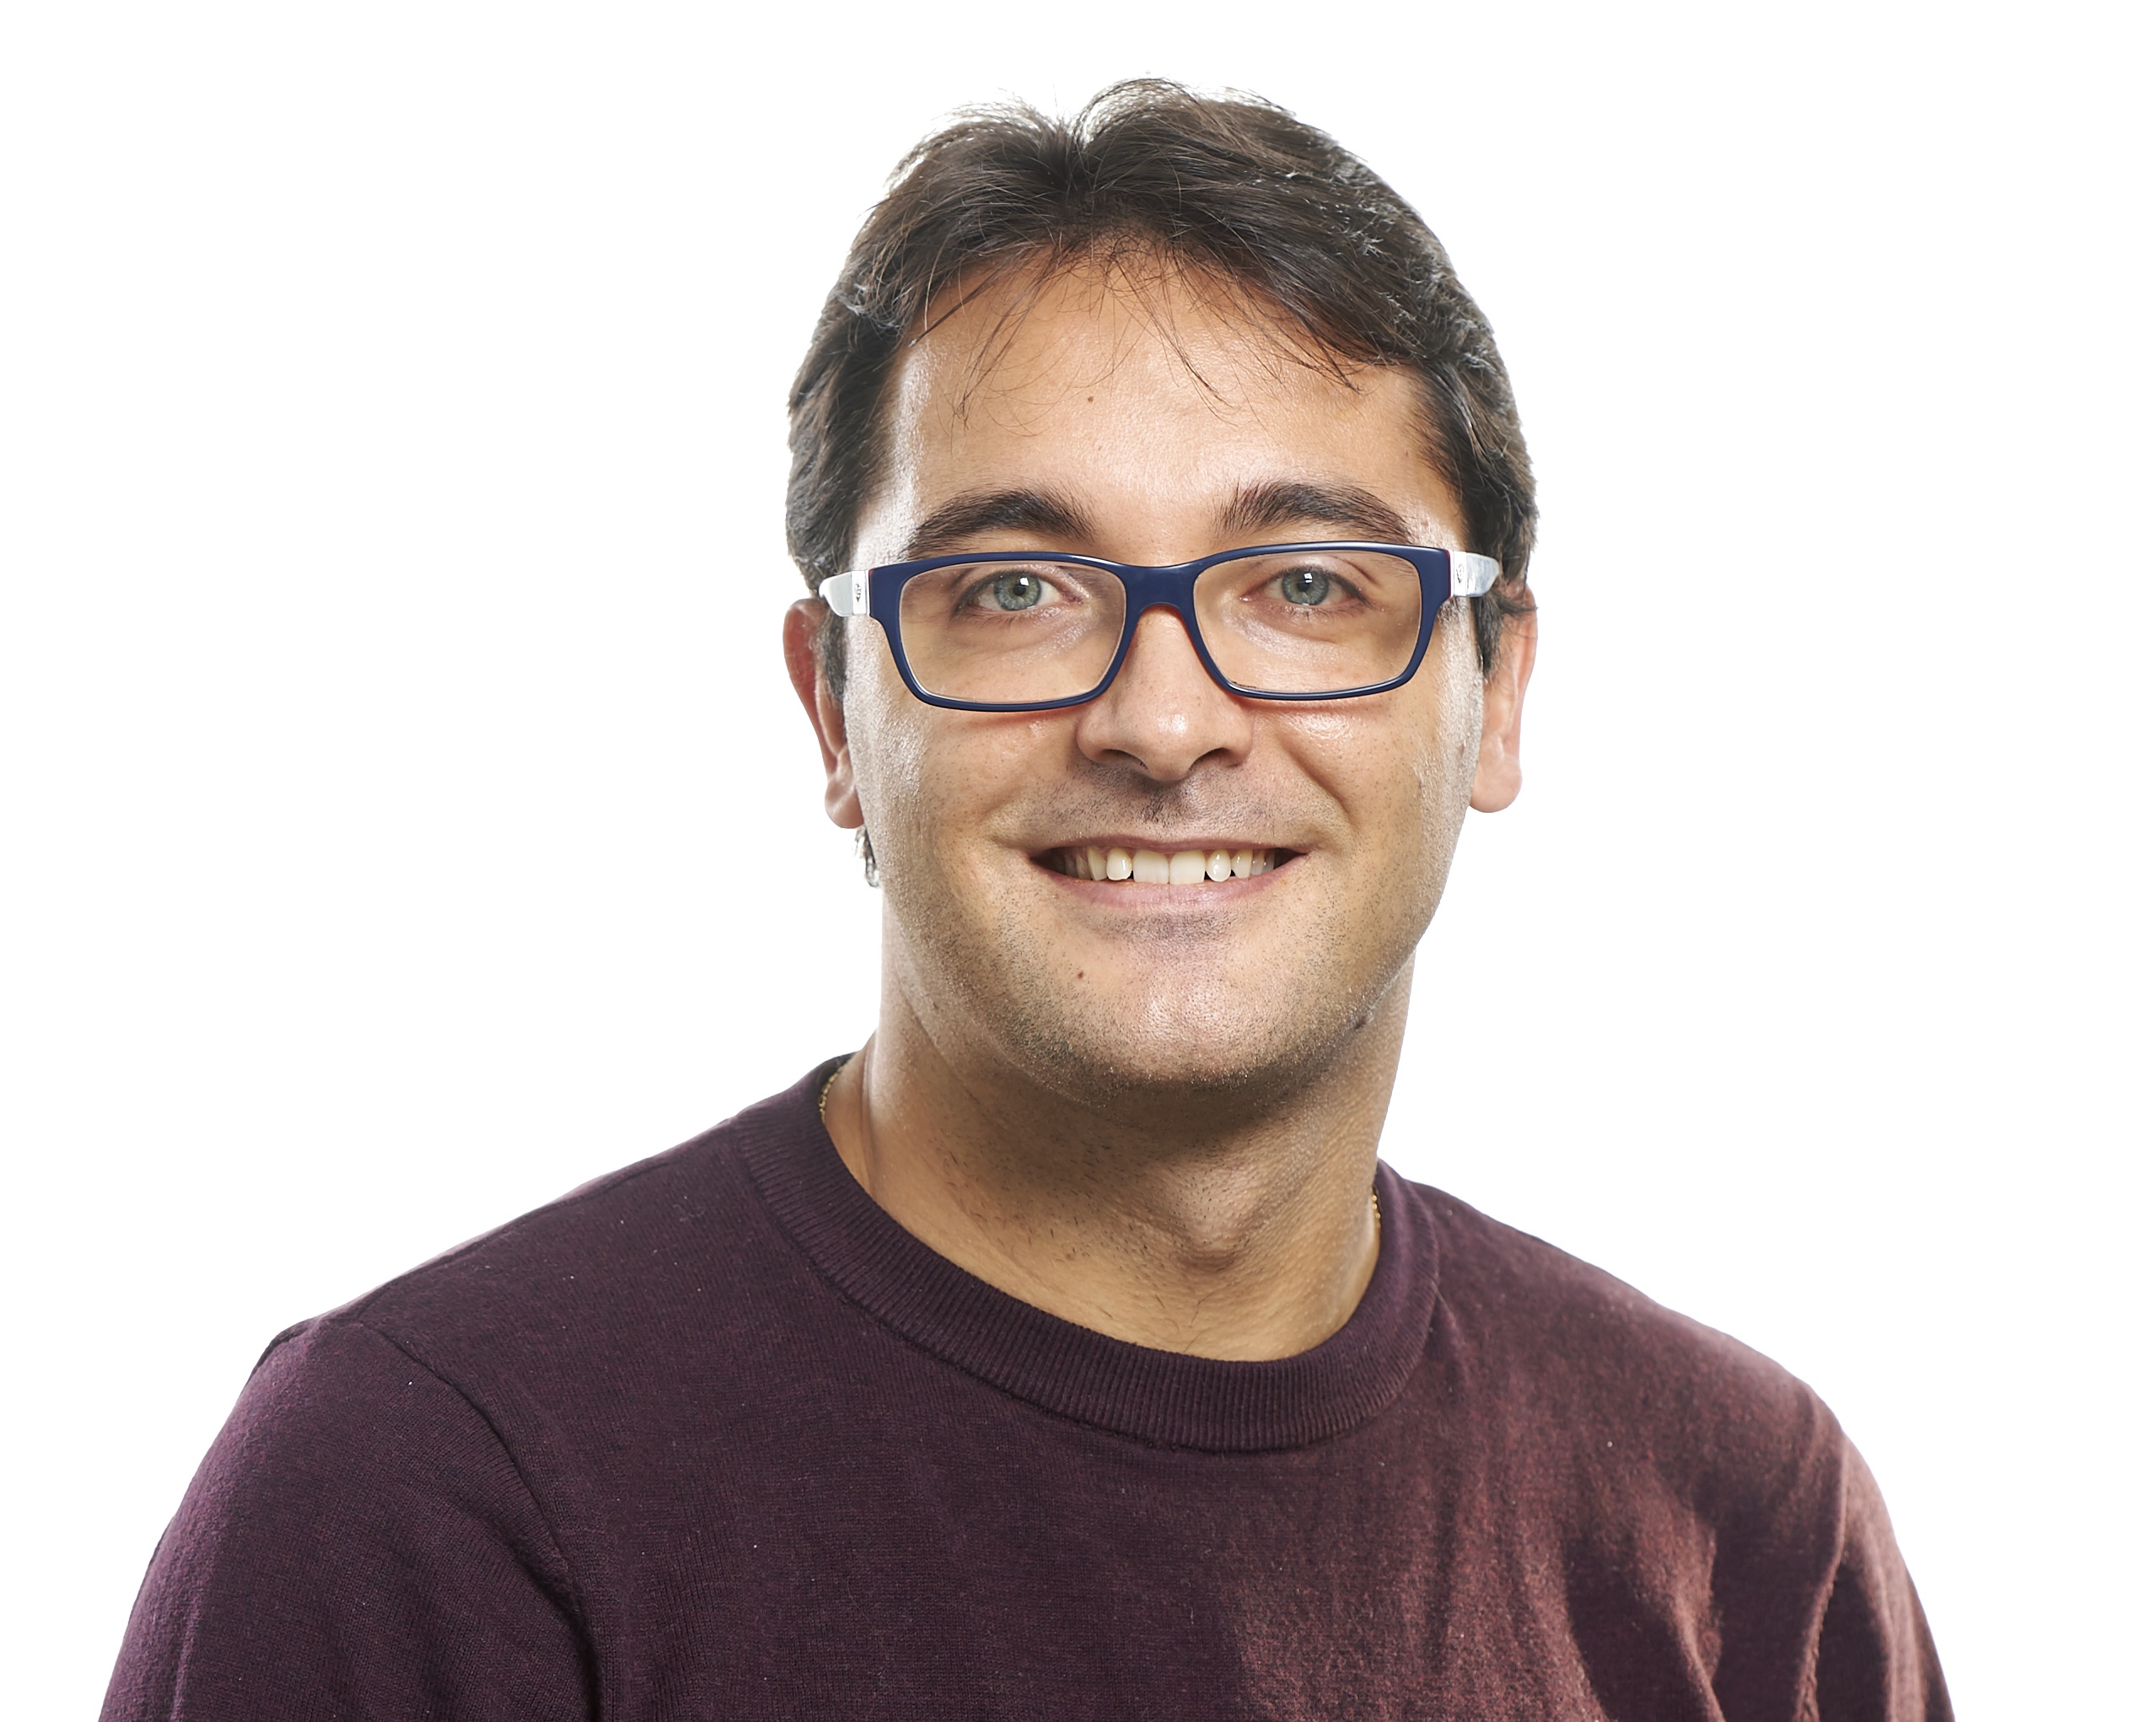
\includegraphics[width=3.3cm, height=3.5cm]{images/s_panichella.jpg}\\
\vspace{-2mm}
\textsc{Sebastiano Panichella - Curriculum vitae}\\
\vspace{-2mm}

%\newlength{\rcollength}\setlength{\rcollength}{1in}%
%\newlength{\spacewidth}\setlength{\spacewidth}{20pt}
%\newcommand\spacechar{$|$}

\noindent\begin{minipage}{0.3\textwidth}% adapt widths of minipages to your needs
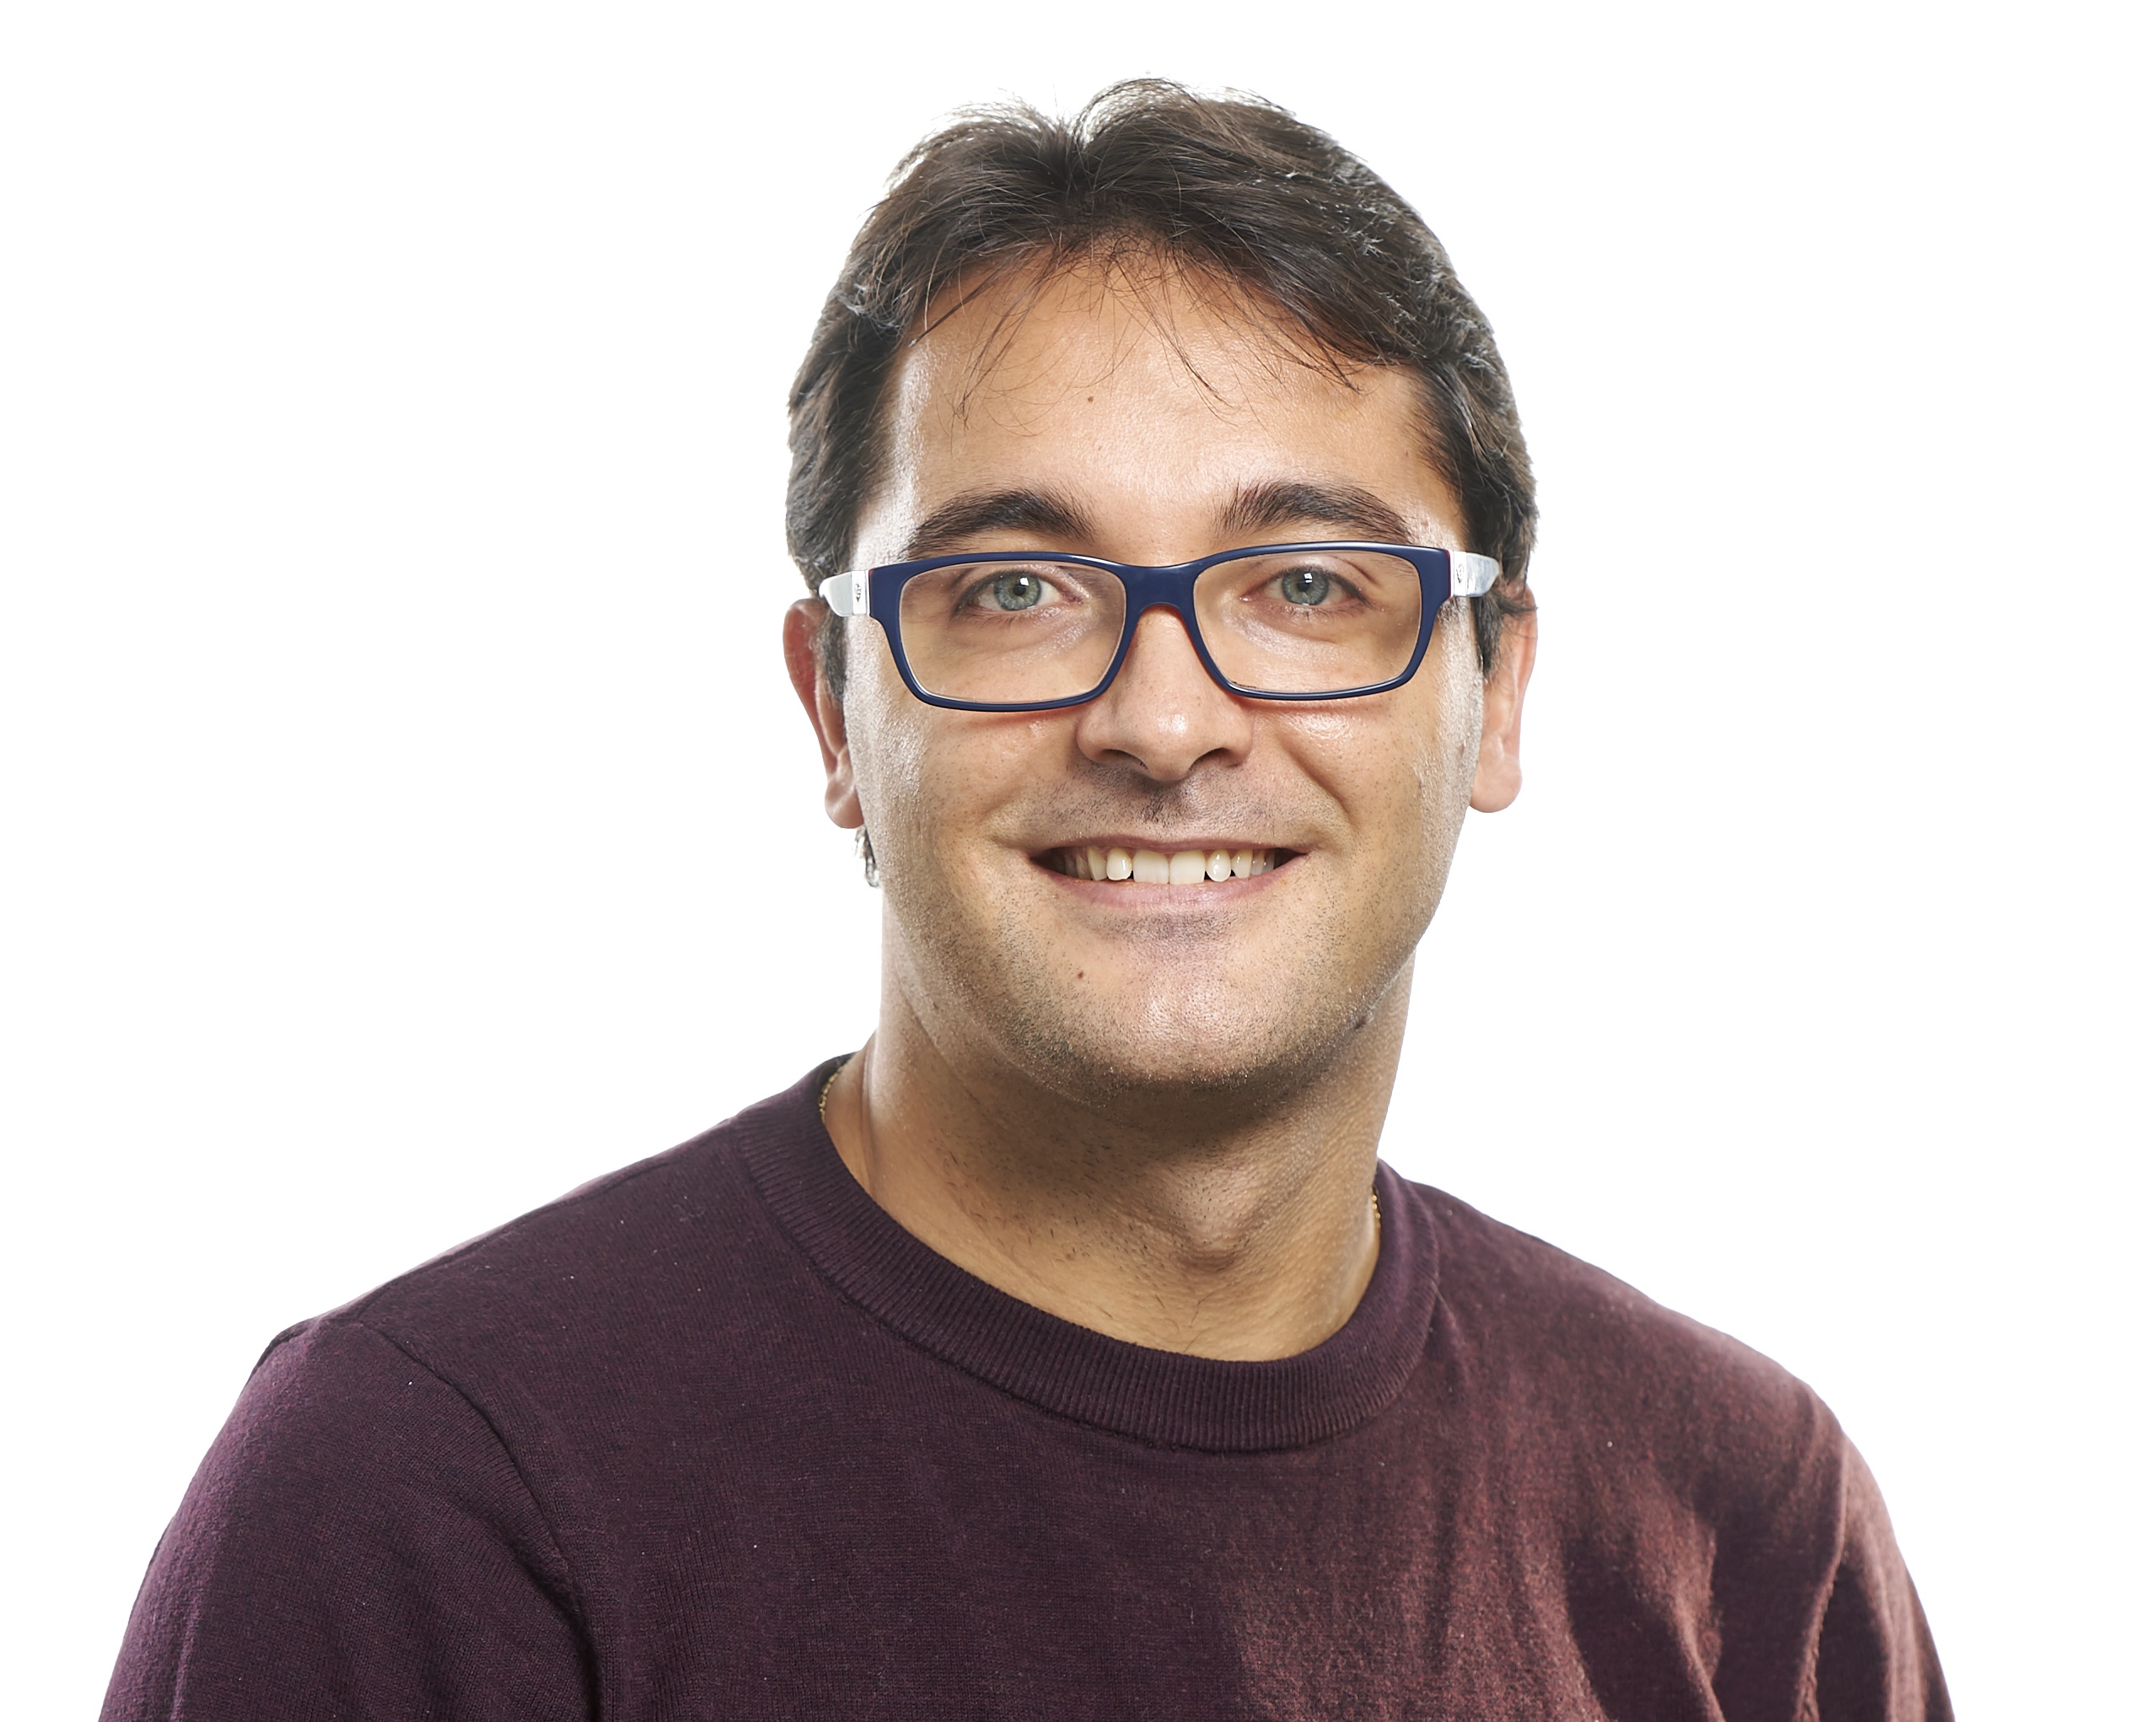
\includegraphics[width=3.3cm, height=3.5cm]{images/s_panichella.jpg}
\end{minipage}%
\hfill%
\begin{minipage}{0.9\textwidth}\raggedright
\textsc{Contact Information}\\
{\small
%\textit{Address:} Department of Computer Engineering\\ \href{http://www.ing.unisannio.it/}{University of Sannio}\\
%RCOST- Palazzo ex Poste, Via Traiano\\
%82100 Benevento (Italy).\\\\
%\textit{Mobile:} +39 3881969673\\
%\textit{Tel.: +39 0824 305539} \\
%\textit{E-mail:} \email{spanichella@gmail.com}\\
%\textit{Home Page:} \href{http://www.ing.unisannio.it/spanichella}{www.ing.unisannio.it/spanichella}
\textit{Address:} School of Engineering,  \href{https://www.zhaw.ch/en/about-us/person/panc/}{Zurich University of Applied Science}\\
Obere Kirchgasse 2 / Steinberggasse 12/14
8400 Winterthur, Switzerland.\\
%\textit{Office: BIN 2.D.03}
%\\ %\textit{Mobile:} +41 788864624\\
%\textit{Tel.: +39 0824 305539} \\
%\textit{Tel +41 44 63 545 78 } \\
\textit{E-mail:} \email{panc@zhaw.ch} (or alternatively \email{spanichella@gmail.com})\\
\textit{Home Page:} \href{https://spanichella.github.io/index.html}{https://spanichella.github.io/index.html}\\
\textit{Google Scholar Ref:}  \url{https://scholar.google.it/citations?user=HiNuBFgAAAAJ\&hl=en\&oi=ao}\\
\textit{Detailed CV:} \href{https://spanichella.github.io/img/CV.pdf}{https://spanichella.github.io/img/CV.pdf}}\\
\end{minipage}


\vspace{2.5mm}
\textsc{EDUCATION}
\vspace{1.5mm}

Sebastiano Panichella was born (19/12/1986) 
in Isernia (Italy), he received (cum laude) the Laurea in Computer Science from the University of Salerno (Italy) in December 2010 defending a thesis on IR-based Traceability Recovery. 
He received the PhD in Computer Science from the University of Sannio (Department of Engineering) defending, in  \textbf{18 July 2014},  the thesis entitled  \href{http://dx.doi.org/10.1109/ICSM.2015.7332519}{\textit{``Supporting Newcomers in Open Source Software Development Projects"}}.  During the PhD his work was supervised by \textbf{\textit{Prof. Massimiliano Di Penta and Prof. Gerardo Canfora}}.

\vspace{2.5mm}
\textsc{Employment history \& Research Goals and Interests}
\vspace{1.5mm}
%During the PhD his work was supervised by 
%Prof. Gerardo Canfora and 
%Prof. Massimiliano Di Penta and Prof. Gerardo Canfora.

%\textbf{Major scientific achievements}
%\vspace{1mm}

Currently he is a (Permanent) Senior Computer Science Researcher at Zurich University of Applied Science (ZHAW), from (\textit{\textbf{20-08-2018}}). Previously he was postdoc at University of Zurich (01-11-2014 - 19-08-2018) working in the lab of Prof. Gall. \\
His main \textbf{research goal} is to conduct industrial research, involving both industrial and academic collaborations, to sustain
the Internet of Things (IoT) vision, where future smart cities will be characterized by millions of smart systems (e.g., cyber-physical
systems) connected over the internet, controlled by complex embedded software implemented for the cloud.\\
His  \textbf{research interests} are in the domain of Software Engineering (SE), cloud computing (CC), and Data Science (DS): DevOps (e.g., Continuous Delivery, Continuous integration), Machine learning applied to SE, Software maintenance and evolution (with particular focus on Cloud, mobile, and Cyber-physical applications), Mobile Computing. Moreover, he is promoting DS research on \textit{Summarization Techniques for Code, Changes, and Testing}. He is a \textbf{member of IEEE}. 
\vspace{1mm}

His research studies involved relevant industrial companies (e.g., ING NEDERLAND, Sony Mobile Communication, SIEMENS, GVM, etc.) and their extensions will involve further industrial organizations and open source projects. He serves and has served as program committee member of various international conference (e.g., ICSE, SBST, ASE, ICPC, ICSME, SANER, MSR, SEAA) and as reviewer for various international journals (e.g., TSE, TOSEM, EMSE, JSS, IST, JSEP) in the fields of software engineering and evolutionary computation. He is currently Editorial Board Member of �\textit{Journal of Software: evolution and process} (JSEP) and Lead (or Co-lead) Guest editor of special issues at EMSE and IST journals.\\

\vspace{1.5mm}
\textsc{Institutional responsibilities}
\vspace{1.5mm}

(Permanent) Senior Computer Science Researcher in Software Engineering (SE), cloud computing (CC), and Data Science (DS) at ZHAW (from 20-08-2018).

%\blankline

%\blankline
%
%\textsc{Research Interests}
%
%%\on{This section should say what *you* are doing in these fields, rather than just defining the fields!}
%
%\textbf{Mining Software Repositories}
%\blankline \\\\
%Software repositories such as source control systems, archived communications between project personnel, and defect tracking systems are used to help manage the progress of software projects. Software practitioners and researchers are recognizing the benefits of mining this information to support the maintenance of software systems, improve software design/reuse, and empirically validate novel ideas and techniques. Research is now proceeding to uncover the ways in which mining these repositories can help to understand software development and software evolution, to support predictions about software development, and to exploit this knowledge concretely in planning future development. The Mining Software Repositories (MSR) field analyzes the rich data available in software repositories to uncover interesting and actionable information about software systems and projects.
%
%   \textbf{Work in progress.}  In past work Panichella focused his attention in mining software repository to build recommender systems for supporting developers during maintenance and program comprehension tasks. For instance, he conceived tools for  (i) enabling the automatic re-documentation of existing systems \ref{C19} \ref{C27};  (ii) summarizing software artifacts \ref{C26} \ref{J5};  (iii) or profiling developers or experts in OSS projects \ref{C12}\ref{C17}\ref{C18}\ref{C20}\ref{C23}\ref{C25}. Currently Panichella is focusing his attention in mining App Store data and data from traditional repositories for designing and developing tools to help  developers digest the huge amount of feedback they receive from users on a daily basis, transforming user reviews into maintenance tasks (fixing issues or building features) \ref{C2}\ref{C3}\ref{C5}\ref{C7}. More in general, he is interested to conceive tools to support developers in evolving modern software applications \ref{C8}\ref{C14}. \\
%
%\textbf{Empirical Software Engineering}
%\blankline\\\\
%Empirical software engineering is a sub-domain of software engineering focusing on experiments on software systems (software products, processes, and resources). It is interested in devising experiments on software, in collecting data from these experiments, and in devising laws and theories from this data. Proponents of experimental software engineering advocate that the nature of software is such that we can advance the knowledge on software through experiments only. The scientific method suggests a cycle of observations, laws, and theories to advance science. Empirical software engineering applies this method to software.
%
%   \textbf{Work in progress.} In past work Panichella performed empirical studies to understand (i) how   OSS communities upgrades dependencies \ref{J2}\ref{C21};   
%   (ii) to what extent static analysis tools help developers with code reviews \ref{C16};  (iii)  how developers' collaborations identified from different sources vary when they are mined from different sources \ref{C17};  (iv) how the evolution of emerging collaborations relates to code changes \ref{C20}; or (v) to study
%   the behaviour of developers during maintenance tasks (e.g., while they modify existing features or fix a bug) by analyzing their navigation patterns  \ref{C22}. Currently Panichella is focusing his attention in performing empirical work to understand possible ways to measure and foster developer  productivity during testing \ref{C10}, maintenance \ref{C22} and code reviewing tasks  \ref{C16}.
%   \\
%   
%\textbf{Code Review}
%\blankline\\\\
%Peer code review, a manual inspection of source code by developers other than the author, is recognized as a valuable tool for reducing software defects and improving the quality of software projects. In 1976, Fagan formalized a highly structured process for code reviewing, based on line-by-line group reviews, done in extended meetings--code inspections. Over the years, researchers provided evidence on code inspection benefits, especially in terms of defect finding, but the cumbersome, time-consuming, and synchronous nature of this approach hinders its universal adoption in practice. Nowadays, many organizations are adopting more lightweight code review practices to limit the inefficiencies of inspections. In particular, there is a clear trend toward the usage of tools specifically developed to support code review. Modern code reviews are (1) informal (in contrast to Fagan-style), (2) tool-based, and (3) occurs regularly in practice nowadays, for example at companies such as Microsoft, Google, Facebook, and in other companies and OSS projects. %The growth in usage of the modern code review process raises many questions.
%
%   \textbf{Work in progress.} The research focus of Panichella is to develop recommender systems able to (better) support developers during the code review process \ref{C16}.
%   \\
%
%\textbf{IR-based Traceability Recovery}
%\blankline\\\\
%Traceability has been defined as "the ability to describe and follow the life of an artefact (requirements, code, tests, models, reports, plans, etc.), in both a forwards and backwards direction". Thus, traceability links help software engineers to understand the relationships and dependencies among various software artefacts (requirements, code, tests, models, etc.) developed during the software lifecycle. The two main research topics related to the traceability management are event-based systems for traceability management and information retrieval based methods and tools supporting the software engineer in the traceability link recovery.\\
%   \textbf{Work in progress.} In past work Panichella explored several enhancing strategies for improving IR-based Traceability Recovery approaches, most of them are based on (i) smoothing filters  \ref{J3} \ref{J4} and (ii)  NLP approaches \ref{C28} \ref{C29} \ref{C30}. Recently Panichella is focusing his effort in tracing link between data and software artifacts stored in modern software repositories \ref{C2}  \ref{C3} \ref{C5}.
%   \\
%
%\textbf{Textual analysis}
%\blankline\\\\
%Textual analysis can be described as the examination of a text in which an educated guess is formed as to the most likely interpretations that might be made of that text. It is where the researcher must decentre the text to reconstruct it, working back through the narrative’s mediations of form, appearance, rhetoric, and style to uncover the underlying social and historical processes, the metalanguage that guided the production. It is suggested that textual analysis can cover four main underlying constructs: language and meaning, ideology, ideology and myth, and historicity. In this sense, textual analysis is a methodology: a way of gathering and analysing information in academic research (Mckee, A 2001).\\
%   \textbf{Work in progress.} Panichella  studied text analysis approaches since his bachelor and master studies and was always fascinated by the great usability of Natural Language Processing (NLP) and Information Retrieval (IR) tools and techniques for solving several practical problems. He adopted such techniques in several work during his PhD and also during the postdoctoral experience. He is currently learning new techniques and tools based on Textual Analysis      (e.g. WORD2VEC) and neural networks techniques \ref{C1}.
%   \\
%
%\textbf{Machine Learning and Genetic Algorithms}
%\blankline\\\\
%Machine learning (ML) and Genetic Algorithms (GA) deals with the issue of how to build computer programs that improve their performance at some tasks through experience. ML and Genetic algorithms have proven to be of great practical value in a variety of application domains. Not surprisingly, the field of software engineering turns out to be a fertile ground where many software development and maintenance tasks could be formulated as learning problems and approached in terms of learning algorithms. 
%   \textbf{Work in progress.} Panichella was also very fascinated by the potential of ML and Genetic Algorithms for solving SE problems. He started to study them during the PhD studies. Examples of the successful application of  ML and genetic algorithms to SE problems by Panichella are  bug prediction, code (and code change) prediction  \ref{C9} \ref{J1} \ref{J3} \ref{C24},  
% prioritization or clustering of user reviews (in the context of mobile apps) \ref{C2}\ref{C3}\ref{C5}\ref{C7}  \ref{C8}\ref{C14}, test case generation \ref{C10}, etc.. Current research interest are toward experimenting customized solutions based on ML and Genetic Algorithms for enhancing traditional testing approaches and GUI testing processes \ref{Cm3}. \\
%   \\
%
%\textbf{ Continuous Delivery}
%\blankline\\\\\
%Continuous delivery (CD) is a software engineering approach in which teams produce software in short cycles, ensuring that the software can be reliably released at any time. It aims at building, testing, and releasing software faster and more frequently. The approach helps reduce the cost, time, and risk of delivering changes by allowing for more incremental updates to applications in production. A straightforward and repeatable deployment process is important for continuous delivery. Continuous Integration (CI) consists in a specific stage of CD process where team members integrate their work in an automatic manner, which allows a fast building, testing, and releasing of software, leading to multiple integrations per day. Researchers in this field have as main focus the development of recommender systems able to provide suggestions to developers and testers during Continuous Integration activities. 
%\\
%   \textbf{Work in progress.}  In the context of CI Panichella is currently conducting empirical work to understand the problems that developers face when integrating new changes in the code base \ref{C0} \ref{Cm3}. The main focus is the development of recommender systems able to provide suggestions to developers and testers during Continuous Integration activities.  \\
%
%\textsc{Academic Appointments} 
%
%Currently 
%%\chg{he}{Panichella}
%Panichella
% is a Research Associate at
%  %\ins{the} 
% the University of Zurich  (\textit{\textbf{since November 2014}})  working in the \href{http://www.ifi.uzh.ch/seal.html}{\textit{Software Evolution and Architecture (SEAL) Lab}} of Prof. Harald Gall.  He is a member of IEEE. His research interests include Mobile Computing, Mining Software Repositories, Code Review, IR-based Traceability Recovery, Textual Analysis, Machine Learning and Genetic Algorithms applied to SE problems, Continuous Delivery (with special attention to Continuous Integration Problems), Software maintenance and evolution and Empirical Software Engineering. He is author of \textbf{39} papers (\textbf{21} of them published during the experience at the SEAL lab) appeared in International Conferences and Journals. These research work involved studies in industrial companies (e.g., ING NEDERLAND, Sony Mobile Communication, etc.) and open source projects and received best paper awards. He serves and has served as program committee member of various international conference (e.g., ICSE, SBST, ASE, ICPC, ICSME, SANER, MSR, SEAA) and as reviewer for various international journals (e.g., TSE, TOSEM, EMSE, JSS, IST, JSEP) in the fields of software engineering and evolutionary computation. He is currently Editorial Board Member of �\textit{Journal of Software: evolution and process} (JSEP).
%
%\textsc{Academic Experience and History}
%
%\href{http://www.ing.unisannio.it/}{\textbf{University of Sannio}}, Italy
%\begin{outerlist}
%\item[] PhD.,
%        \href{http://www.ing.unisannio.it/}
%             {Computer Engineering}, June/July 2014
%        \begin{innerlist}
%        %\bigsqcup
%        \item Thesis Title: \emph{\href{http://www.ifi.uzh.ch/seal/people/panichella/Dissertation_Sebastiano_Panichella.pdf}{\textit{``Supporting Newcomers in Open Source Software Development Projects"}}}
%        \item Advisers:
%             \href{www.gerardocanfora.net/‎}
%                   {Prof. Gerardo Canfora} and
%              \href{www.rcost.unisannio.it/mdipenta/}
%                   {Prof. Massimiliano Di Penta}
%        \item Thesis Topics: Supporting Developers, Mining of Software Repositories (Mailing lists, Issue trackers, Versioning Systems etc.)\\
% \end{innerlist}
%\end{outerlist}
%
%\href{http://www.unisa.it/}{\textbf{University of Salerno}}, Italy
%\begin{outerlist}
%\item[] M.S.,
%        \href{http://www.unisa.it/facolta/scienze_mmffnn/index}
%             {Computer Science}, December 2010
%        \begin{innerlist}
%        \item \emph{Magna cum Laude}
%        \item Thesis Title: \emph{Improving IR-based Traceability Recovery Using Smoothing Filters}
%        \item Adviser:
%              \href{http://www.dmi.unisa.it/people/delucia/www/}
%                   {Prof. Andrea De Lucia}
%        \item Thesis Topics: Software Engineering, Traceability Recovery, Textual Analysis\\
% \end{innerlist}
%\end{outerlist}
%
%
%\href{http://www.unimol.it/}{\textbf{University of Molise}}, Italy
%\begin{outerlist}
%
%\item[] B.S.,
%        \href{http://www.unimol.it/pls/unimolise/v3_s2ew_consultazione.mostra_pagina?id_pagina=51098}
%             {Computer Science}, October 2008
%        \begin{innerlist}
%        \item \emph{Magna cum Laude}
%        \item Thesis Title: \emph{Improving IR-based traceability recovery via noun-based indexing of software artifacts}
%        \item Advisers:
%              \href{http://docenti.unimol.it/index.php?u=giovanni.capobianco}
%                   {Prof. Giovanni Capobianco},
%              \href{http://www.distat.unimol.it/people/oliveto/Home.html}
%                   {Dr Rocco Oliveto}
%        \item Thesis Topics: Software Engineering, Traceability Management, Natural Language Processing (NLP)
%        \end{innerlist}
%
%\end{outerlist} 
%
%\blankline
%
%\textsc{Refereed Journal Publications}
%In papers marked with (*)  the authors are listed in alphabetic order. %When such a rule is not followed, authors are listed by contribution.
%\textbf{\\\underline{Journal Publications during the postdoctoral experience:}}\\
%\begin{bibenum}
%
%\item \label{J1} G. Canfora, A. De Lucia, M. Di Penta, R. Oliveto, A. Panichella, \underline{S. Panichella}. \textbf{*Defect Prediction as a Multi-Objective Optimization Problem}. \emph{Software Testing, Verification and Reliability (STVR)} 2015.\\
%    \doi{10.1002/stvr.1570}\\
%  \end{bibenum}
%  
%  \textbf{\\\underline{Journal Publications during the PhD study:}}\\
%  \begin{bibenum}
%    \item \label{J2} G. Bavota, G. Canfora, M. Di Penta, R. Oliveto, \underline{S. Panichella}. \textbf{*How the Apache Community Upgrades Dependencies}. \emph{Empirical Software Engineering (EMSE)} 2014.\\
%             \doi{10.1007/s10664-014-9325-9}
%             
%    \item \label{J3}  A. De Lucia, M. Di Penta, R. Oliveto, A. Panichella, \underline{S. Panichella}. \textbf{*Applying a Smoothing Filter to Improve IR-based Traceability Recovery Processes: An Empirical Investigation}. \emph{Information and Software Technology (INFSOF)} 2012.\\
%        \doi{10.1016/j.infsof.2012.08.002}
%
%    \item \label{J5} A. De Lucia, M. Di Penta, R. Oliveto, A. Panichella, \underline{S. Panichella}. \textbf{*Labeling Source Code with Information Retrieval Methods: An Empirical Study}. \emph{Empirical Software Engineering (EMSE)} 2013.
%                \doi{doi:10.1007/s10664-013-9285-5}
%        %       To Appear.\\
%\end{bibenum} 
%
%  \textbf{\\\underline{Journal Publications during the master study:}}\\
%\begin{bibenum}
%    \item \label{J4}  G. Capobianco, A. De Lucia, R. Oliveto, A. Panichella, \underline{S. Panichella}. \textbf{*Improving IR-based traceability recovery via noun-based indexing of software artifacts}. \emph{Journal of Software: Evolution and Process (JSE)} 2012.\\
%        \doi{10.1002/smr.1564}
%
%\end{bibenum} 
%%\textsc{Submitted Journal Publications}
%%\begin{bibenum}
%%     \item     \underline{S. Panichella} Harald Gall. \textbf{Recommending Mentors in Open Source Projects to Grow-Up Long Term Contributors}. In: \emph{JSEP}\\
%%\end{bibenum}
%
%%\blankline   
%
%
% 
%\blankline
%
%\textsc{Conference Publications}
%In papers marked with (*)  the authors are listed in alphabetic order. %When such a rule is not followed, authors are listed by contribution.
%
%\textbf{\\\underline{Conference Publications during the postdoctoral experience:}}\\
%\begin{bibenum}
%
%      \item \label{Cm3}  G. Grano, A. Ciurumelea, \underline{S. Panichella}, F. Palomba, H. Gall. \textbf{ Exploring the Integration of User Feedback in Automated Testing of Android Applications.}.  \emph{Proceedings of the  {IEEE} 25th International Conference on Software Analysis, Evolution
%               and Reengineering}  (SANER 2018) - To Appear. \textit{Core RANK: B}.
%
%
%      \item \label{Cm2}  C. Vassallo, \underline{S. Panichella}, F. Palomba, S. Proksch, A. Zaidman and H. Gall. \textbf{Context is King: The Developer Perspective on the Usage of Static Analysis Tools.}.  \emph{Proceedings of the  {IEEE} 25th International Conference on Software Analysis, Evolution
%               and Reengineering}  (SANER 2018) - To Appear. \textit{Core RANK: B}.
%
%
%      \item \label{Cm1}  G. Grano, A. Di Sorbo, F. Mercaldo, C. Visaggio, G. Canfora, \underline{S. Panichella}. \textbf{Android Apps and User Feedback: a Dataset for Software Evolution and Quality Improvement.}.  \emph{Proceedings of the  International Workshop on App Market Analytics}  (WAMA 2017). 
%
%      \item \label{C0}  C. Vassallo, G. Schermann, F. Zampetti, D. Romano, P. Leitner, A. Zaidman, M. di Penta, \underline{S. Panichella}.
%         \textbf{A Tale of CI Build Failures: an Open Source and a Financial Organization Perspective.}.  \emph{Proceedings of the 33rd International Conference on Software Maintenance and Evolution}  (ICSME 2017). \textit{Core RANK: A}.
%      \item \label{C1}  C. V. Alexandru, \underline{S. Panichella}, Harald Gall.
%         \textbf{Replicating Parser Behavior using Neural Machine Translation}.  \emph{Proceedings of the 25th International Conference on Program Comprehension} (ICPC 2017). \textit{Core RANK: B}.
%
%      \item \label{C2}  A. Di Sorbo,  \underline{S. Panichella}, C. V. Alexandru, C. A. Visaggio, G. Canfora.
%         \textbf{SURF: Summarizer of User Reviews Feedback}.  Demonstrations Track of the  \emph{39th International Conference on Software Engineering} (ICSE 2017). \textit{Core RANK: A*}.
%
%\item  \label{C3} F. Palomba, P. Salza, A. Ciurumelea,  \underline{S. Panichella}, H. Gall, F. Ferrucci,  A. De Lucia   \textbf{Recommending and Localizing Change Requests for Mobile Apps based on User Reviews}.    In: \emph{39th International Conference on Software Engineering} (ICSE 2017).  \textit{Core RANK: A*}.
%
%         \item  \label{C4} Y. Zhou, R. Gu, T. Chen, Z. Huang,  \underline{S. Panichella}, H. Gall.   \textbf{Analyzing APIs Documentation and Code to Detect Directive Defects}.    In: \emph{39th International Conference on Software Engineering} (ICSE 2017).  \textit{Core RANK: A*}.
%       \item   \label{C5}    A. Ciurumelea, A. Schaufelbuhl, \underline{S. Panichella}, Harald Gall. \textbf{ Analyzing Reviews and Code of Mobile Apps for better Release Planning}. In: \emph{Proceedings of the 24th IEEE International Conference on Software Analysis, Evolution, and Reengineering (SANER) 2017. Klagenfurt, Austria}.  \textit{Core RANK: B}.
%                \item   \label{C6}    C. Alexandru,  \underline{S. Panichella}, Harald Gall. \textbf{Reducing Redundancies in Multi-Revision Code Analysis}. In: \emph{24th IEEE International Conference on Software Analysis, Evolution, and Reengineering  (SANER) 2017. Klagenfurt, Austria}.  \textit{Core RANK: B}.
%              
%    \item  \label{C7}  \underline{S. Panichella}, A. Di Sorbo, E. Guzman, C. Visaggio, G. Canfora, H. Gall.
%         \textbf{ARdoc: App Reviews Development Oriented Classifier}.  In: \emph{24th ACM SIGSOFT International Symposium on the Foundations of Software Engineering}  will be held in Seattle, WA, USA.  \textit{Core RANK: A*}.
%  
%      \item  \label{C8}  A. Di Sorbo,  \underline{S. Panichella}, C. V. Alexandru, J. Shimagaki, C. A. Visaggio, G. Canfora, H. Gall.
%         \textbf{What Would Users Change in My App? Summarizing App
%Reviews for Recommending Software Changes}.  In: \emph{24th ACM SIGSOFT International Symposium on the Foundations of Software Engineering}  will be held in Seattle, WA, USA.  \textit{Core RANK: A}.
%         \item  \label{C9}  A. Panichella, C. Alexandru,  \underline{S. Panichella}, A. Bacchelli, H. Gall. \textbf{A Search-based Training Algorithm for Cost-aware Defect Prediction}.  \emph{25th International Conference on Genetic Algorithms (ICGA) and the 21st Annual Genetic Programming Conference (GP) (GECCO 2016)}.  Denver, Colorado, USA.  \textit{Core RANK: A}.
%        
%    \item  \label{C10}   \underline{S. Panichella}, A. Panichella, M. Bella, A. Zaidman, H. Gall. \textbf{The impact of test case summaries on bug fixing performance: An empirical investigation}. In: \emph{Proceedings of the 38th International Conference on Software Engineering} (ICSE 2016), Austin, TX.  \textit{Core RANK: A*}.
%
%    \item   \label{C11}   A. Di Sorbo, \underline{S. Panichella}, C. Visaggio, M. Di Penta, G. Canfora,  H. Gall. . \textbf{DECA: Development Emails Content Analyzer}. In: \emph{Proceedings of the 38th International Conference on Software Engineering} (ICSE 2016), Austin, TX.  \textit{Core RANK: A*}.
%
%    \item  \label{C12}   \underline{S. Panichella}. \textbf{Supporting Newcomers in Software Development Projects}. In: \emph{Proceedings of the 31st International Conference on Software Maintenance and Evolution} (ICSME 2015). Bremen, Germany.  \textit{Core RANK: A}.
%
%        \item  \label{C13}  A. Di Sorbo, \underline{S. Panichella}, C. Visaggio, M. Di Penta, G. Canfora,  H. Gall. \textbf{Development Emails Content Analyzer: Intention Mining in Developer Discussions}. In: \emph{30th international conference on Automated Software Engineering} (ASE 2015).  Lincoln, Nebraska.  \textit{Core RANK: A}.
%
%    \item  \label{C14}   \underline{S. Panichella}, A. Di Sorbo, E. Guzman, C. Visaggio, G. Canfora, H. Gall. \textbf{How Can I Improve My App? Classifying User Reviews for Software Maintenance and Evolution}. In: \emph{Proceedings of the 31st International Conference on Software Maintenance and Evolution} (ICSME 2015). Bremen, Germany.  \textit{Core RANK: A}.
%
%    \item  \label{C15}  G. Schermann, M. Brandtner,  \underline{S. Panichella}, P. Leitner,  H. Gall. \textbf{Discovering Loners and Phantoms in Commit and Issue Data}. In: \emph{Proceedings of the 37th International Conference on Program Comprehension} (ICPC 2015). Firenze, Italy.  \textit{Core RANK: C}.
%
%
%    \item   \label{C16}  \underline{S. Panichella}, V. Arnaoudova, M. Di Penta, G. Antoniol. \textbf{Would Static Analysis Tools Help Developers with Code Reviews?}.  In: \emph{Proceedings of the 22nd International Conference on Software Analysis, Evolution and Reengineering} (SANER 2015). Montreal, Canada.  \textit{Core RANK: B}.
%
%\end{bibenum}
%
%\textbf{\\\underline{Conference Publications during the PhD experience:}}\\
%\begin{bibenum}
%    \item  \label{C17}  \underline{S. Panichella}, G. Bavota, M. Di Penta, G. Canfora, G. Antoniol. \textbf{How Developers' Collaborations Identified from Different Sources Tell us About Code Changes}. In: \emph{Proceedings of the 30th International Conference on Software Maintenance and Evolution} (ICSME 2014). Victoria, Canada.  \textit{Core RANK: A}.
%
%    \item  \label{C18}  G. Bavota, \underline{S. Panichella}, N. Tsantalis, M. Di Penta, R. Oliveto, G. Canfora. \textbf{Recommending Refactorings based on Team Co-Maintenance Patterns.}. In: \emph{29th international conference on Automated Software Engineering} (ASE 2014). Vasteras, Sweden.  \textit{Core RANK: A}.
%
%    \item  \label{C19}  C. Vassallo, \underline{S. Panichella}, G. Canfora, M. Di Penta. \textbf{CODES: mining sourCe cOde Descriptions from developErs diScussions}. In: \emph{Proceedings of the 36th International Conference on Program Comprehension} (ICPC 2014). Hyderabad, India.  \textit{Core RANK: B}.
%
%    \item  \label{C20}  \underline{S. Panichella}, G. Canfora, M. Di Penta, R. Oliveto. \textbf{How the Evolution of Emerging Collaborations Relates to Code Changes: an Empirical Study}. In: \emph{Proceedings of the 36th International Conference on Program Comprehension} (ICPC 2014). Hyderabad, India.  \textit{Core RANK: B}.
%
%    \item  \label{C21}  G. Bavota, G. Canfora, M. Di Penta, R. Oliveto, \underline{S. Panichella}. \textbf{*The Evolution of Project Inter-Dependencies in a Software Ecosystem: the Case of Apache}. In: \emph{Proceedings of the 29th International Conference on Software Maintenance} (ICSM 2013). Eindhoven, Netherlands.  \textit{Core RANK: A}.
%
%    \item  \label{C22}  G. Bavota, G. Canfora, M. Di Penta, R. Oliveto, \underline{S. Panichella}. \textbf{*An Empirical Investigation on Documentation Usage Patterns in Maintenance Tasks}. In: \emph{Proceedings of the 29th International Conference on Software Maintenance} (ICSM 2013). Eindhoven, Netherlands.  \textit{Core RANK: A}.
%
%    \item  \label{C23}  G. Canfora, M. Di Penta, S. Giannantonio, R. Oliveto,  \underline{S. Panichella}. \textbf{*YODA: Young and newcOmer Developer Assistant}. In: \emph{Proceedings of the 35th International Conference on Software Engineering} (ICSE 2013). San Francisco, CA, USA.  \textit{Core RANK: A*}.
%
%     \item  \label{C24}  G. Canfora, A. De Lucia, M. Di Penta, R. Oliveto, A. Panichella, \underline{S. Panichella}. \textbf{*Multi-Objective Cross-Project Defect Prediction}. In: \emph{Proceedings of the 7th International Conference on Software Testing, Verification and Validation} (ICST 2013). Luxembourg.  \textit{Core RANK: A}.
%
%     \item   \label{C25}  G. Canfora, M. Di Penta, R. Oliveto,  \underline{S. Panichella}. \textbf{*Who is going to Mentor Newcomers in Open Source Projects?}. In: \emph{Proceedings of the 29th ACM SIGSOFT International Symposium on Foundations of Software Engineering} (FSE 2012). Cary, North Carolina, USA.  \textit{Core RANK: A*}.
%
%     \item  \label{C26} A. De Lucia, M. Di Penta, R. Oliveto, A. Panichella, \underline{S. Panichella}. \textbf{*Using IR Methods for Labeling Source Code Artifacts: Is It Worthwhile?}. In: \emph{Proceedings of the 20th IEEE International Conference on Program Comprehension} (ICPC), 2012. Passau, Germany.  \textit{Core RANK: B}.
%
%     \item  \label{C27}  \underline{S. Panichella}, J. Aponte, M. Di Penta, A. Marcus, G. Canfora. \textbf{Mining source code descriptions from developer communications}. In: \emph{Proceedings of the 20th IEEE International Conference on Program Comprehension} (ICPC), 2012. Passau, Germany.  \textit{Core RANK: B}.
%
%     \item  \label{C28}  A. De Lucia, M. Di Penta, R. Oliveto, A. Panichella, \underline{S. Panichella}. \textbf{*Improving IR-based Traceability Recovery Using Smoothing Filters}. In: \emph{Proceedings of the 19th IEEE International Conference on Program Comprehension} (ICPC) 2011. Kingston, ON, Canada.  \textit{Core RANK: B}.
%
%\end{bibenum}
%
%\textbf{\\\underline{Conference Publications during the bachelor and master studies:}}\\
%\begin{bibenum}
%     \item  \label{C29}  G. Capobianco, A. De Lucia, R. Oliveto, A. Panichella, \underline{S. Panichella}. \textbf{*On the role of the nouns in IR-based traceability recovery}. In: \emph{Proceedings of the 19th IEEE International Conference on Program Comprehension} (ICPC) 2009. Vancouver, British Columbia, Canada.  \textit{Core RANK: B}.
%
%     \item  \label{C30}  G. Capobianco, A. De Lucia, R. Oliveto, A. Panichella, \underline{S. Panichella}. \textbf{*Traceability Recovery Using Numerical Analysis}. In: \emph{Proceedings of the 16th IEEE Working Conference on Reverse Engineering} (WCRE) 2009. Lille, France.  \textit{Core RANK: B}.
%     
%\end{bibenum}


%\blankline

%\textsc{Submitted Papers}
%In papers marked with (*)  the authors are listed in alphabetic order. When such a rule is not followed, authors are listed by contribution.
%\begin{bibenum}
%      \item A. Di Sorbo,  \underline{S. Panichella}, C. V. Alexandru, J. Shimagaki, C. A. Visaggio, G. Canfora, H. Gall.
%         \textbf{What Would Users Change in My App? Summarizing App
%Reviews for Recommending Software Changes}.  In: \emph{24th ACM SIGSOFT International Symposium on the Foundations of Software Engineering}  will be held in Seattle, WA, USA
%\end{bibenum}

%\textsc{Submitted Papers}
%\begin{bibenum}
    %     \item \underline{S. Panichella}, H. Gall.       \textbf{Summarization Techniques for Code, Changes, and Testing}.  Technical Briefing proposal at  the  \emph{39th International Conference on Software Engineering} (ICSE 2017).
      
%                              \item C. Vassallo, F. Zampetti, D. Romano,  \underline{S. Panichella}, M. Di Penta and A. Zaidman  \textbf{What Types of Build Failures Stop Continuous Delivery? An Empirical Study at ING NL}.    In: \emph{39th International Conference on Software Engineering} (ICSE 2017).
 

%\end{bibenum} 


\vspace{2.5mm}


\textsc{Approved research projects}
\vspace{1.5mm}


%\on{Why are you using href for the entire text?}\\
\textbf{EU projects}
\begin{innerlist}
\item Sebastiano Panichella is the technical coordinator for the EU H2020-ICT-2018-20 call, entitled COSMOS, contract no. 957254. \textbf{Description}: Much of the increasing complexity of ICT systems is being driven by the more distributed and heterogeneous nature of these systems, with Cyber-Physical Systems accounting for an increasing portion of Software Ecosystems. This basic premise underpins the COSMOS proposal which focuses on blending best practices DevOps solutions with the development processes used in the CPS context: this will enable the CPS world to deliver software more rapidly and result in more secure and trustworthy systems. COSMOS brings together a balanced consortium of big industry, SMEs and academics which will develop enhanced DevOps pipelines which target development of CPS software.
The COSMOS CPS pipelines will be validated against 5 use cases provided by industrial partners representing healthcare, avionics, automotive, utility and railway sectors. These will act as reference use cases when promoting the technology amongst Open Source and standardization communities. For the former a specific community building activity will be performed to stimulate engagement with Open Source; for the latter, the standards experience of the coordinator and partners will be employed to promote COSMOS technologies within heavily regulated sectors where there is an increasing need for well-defined software V\&V solutions. 
\textbf{Total H2020 project 5MIL EUR, Sebastiano Panichella got direct funding for 770,000 EUR} 
   \item Sebastiano Panichella was 
   %\ins{was}
    partially funded with Gabriele Bavota, Gerardo Canfora, Massimiliano Di Penta, in the \href{��http://www.markosproject.eu/��}
                   {EU FP7-ICT-2011-8 project Markos}, contract no. 317743. Specifically, the MARKOS project aimed to realize the prototype of a service and an interactive application providing an integrated view on the Open Source projects available the on web, focusing on functional, structural and licenses aspects of software code. 
                   %My effort is focused on implementing relevant aspects of the Software System realized by Markos and and a generate new research results in the field of Software Engineering. Particular effort is spent on analysis of source code to study the evolution of software project to automatically extract reusable components from source code. From the other things I also extract licensing statements from the source code to monitor their evolution and avoid that changes in source code also generate the break of licenses.
\end{innerlist}
\newpage
\textbf{Innosuisse projects}
\begin{innerlist}
   \item Sebastiano Panichella is the main research responsible of Innosuisse project ARIES: Exploiting User Journeys for Supporting Mobility as a Service Platforms (project Nr. 45548.1 IP-ICT).
ARIES brings together a consortium of two partners: the start-up BOND (\href{https://bond.info/en/}{https://bond.info/en/}) and the ZHAW.
ARIES project will deliver a user-oriented self-adaptive software platform that implements requirements and testing engineering mechanisms to enhance customer experience. ARIES project will be realized in the context of BOND, a Swiss e-bike sharing start-up.\\
\textbf{Total project funding:} Sebastiano Panichella got direct funding for around \textbf{500,000 CHF}\\
\textbf{Ack:} We personally thank the team of BOND for the very productive and constant research meetings. 
\end{innerlist}

\textbf{SNF projects}
\begin{innerlist}
   \item Sebastiano Panichella obtained funding  (as co-applicant) for
   %\chg{funded}{obtained funding for} 
   the SURF-MobileAppsData SNF (No. 200021$-$166275) project. The goal of the SURF-MobileAppsData project is mining mobile apps data available in app stores to support software engineers in better supporting maintenance and evolution activities for these apps (\textbf{Total SNSF (CHF) 349,926}). \\See page: \href{http://www.ifi.uzh.ch/en/seal/people/panichella/SNF-Projects.html}{http://www.ifi.uzh.ch/en/seal/people/panichella/SNF-Projects.html}
\end{innerlist}

\vspace{6.5mm}


\textsc{Supervision (or Co-Supervision) of junior researchers at graduate and postgraduate level:}\\\\
He is \textbf{supervising, supervised (or co-supervised)} 9 undergrad students, 11 MSc students and  9 PhD students and 5 research assistants, which published in relevant conference and journal venues in Software Engineering. A more complete and updated information on advised researchers at different levels can be found: \href{https://spanichella.github.io/\#teaching}{https://spanichella.github.io/\#teaching}\\
\vspace{1.5mm}
%
%\begin{bibsection}
%
%\item \textbf{Sajad Khatiri, PhD student at Zurich University of Applied Science, Switzerland (from 2021}).
%
%\item \textbf{Pooja Rani, PhD student at University of Bern, Switzerland (from 2018}).\\ 
%       \textit{\textbf{Paper accepted} at SANER 2021}.
%       
%\item \textbf{Muhammad Ilyas Azeem, PhD student at Laboratory for Internet Software Technologies}.\\
%       %\textit{\textbf{PhD main topic(s)}: (i) Reducing Redundancies in Multi-Revision Code Analysis; (ii) Exploring Deep Learning Techniques for Supporting the Mining of information in Structured and Unstructured Data}. 
%       \textit{\textbf{Paper accepted} at ICSSP 2020}.
%
%\item \textbf{Carol V. Alexandru, PhD student at University of Zurich}.\\
%       %\textit{\textbf{PhD main topic(s)}: (i) Reducing Redundancies in Multi-Revision Code Analysis; (ii) Exploring Deep Learning Techniques for Supporting the Mining of information in Structured and Unstructured Data}. 
%       \textit{\textbf{Papers accepted} at GECCO 2016, FSE 2016, SANER 2017, ICPC 2017}.
%       %\textit{\textbf{Co-supervised with Prof. Gall during 2015-2018}}
%\vspace{-1.5mm}
%         \item \textbf{Giovanni Grano, PhD student at University of Zurich}.
%                \\
%       %\textit{\textbf{PhD main topic(s)}: Automated Testing}.
%       \textit{\textbf{Papers accepted} at WAMA 2017, SANER 2018, MaLTeSQuE 2018, JSEP 2019, TSE 2020, JSEP 2020}.
%       %\textit{\textbf{2017-2018}}
%\vspace{-1.5mm}
%         \item \textbf{Adelina Ciurumelea, PhD student at University of Zurich}.\\
%       %\textit{\textbf{PhD main topics}: (i) Mobile Computing; (ii)  NLP and Textual analysis in SE}.
%       \textit{\textbf{Papers accepted} at ICSE 2017, SANER 2017}. 
%       %\textit{\textbf{Supervised between 2016-2018}}
%\vspace{-1.5mm}
%\item \textbf{Carmine Vassallo, PhD student at University of Zurich}.\\
%       %\textit{\textbf{PhD main topic(s)}: Continuous Delivery (CD)}.
%       \textit{\textbf{Papers accepted} at ICSME 2017, SANER 2018, 2 EMSE 2019 and 2020}.
%       %\textit{\textbf{Supervised between 2016-2018}}
%\vspace{-1.5mm}
%\item \textbf{Gerald Schermann, PhD student at University of Zurich}.\\
%       %\textit{\textbf{PhD main topics}: (i) Continuous Delivery (CD); (ii)  Release Engineering}. 
%       \textit{\textbf{Paper accepted} at ICPC 2015}.       %\textit{\textbf{Co-supervised in a ICPC 2015 submission with Dr. Philipp Leitner}}
%\vspace{-1.5mm}
%\item \textbf{Andrea Di Sorbo, PhD student at University of Sannio}.
% \\
%       %\textit{\textbf{PhD main topic(s)}: (i) Mining unstructured data with NLP strategies}.
%       \textit{\textbf{Papers accepted} at 
%       ICSME 2015, ASE 2015, ICSE 2016, FSE 2016}. 
%       %\textit{\textbf{Co-supervised with Prof. Canfora 2015-2018}}
%
%
%%-  University of Zurich: \textbf{Carol  Alexandru}, \textbf{Giovanni Grano}, \textbf{Adelina Ciurumelea}, \textbf{Carmine Vassallo}, \textbf{Gerald Schermann}\blankline\\
%%-  University of Sannio: \textbf{Andrea Di Sorbo}
%%
%\end{bibsection}
%
%\vspace{3.5mm}
%
%\textsc{Master Students Supervised}:
%
%\vspace{1mm}
%
%%-  University of Zurich: \textbf{Timofey Titov, Alessandro Rigamonti, Te Tan, Simon Taennler}.\blankline\\
%%-  University of Sannio: \textbf{Carmine Vassallo}
%- \textbf{Xiao'ao Song, Master student at UZH}. \\
%- \textbf{Neeraj Kumar, Master student at UZH}. \\
%- \textbf{Bill Bosshard, Master student at UZH}. \\
%- \textbf{Atif Ghulam, Master student at UZH}. \\
%- \textbf{Rafael Kallis, Master student at UZH}. \textit{Paper accepted at ICSME 2019 and SCP Journal 2020}.\\
%- \textbf{Timofey Titov, Master student at UZH}.           %\textit{Advised on a master thesis related to the adoption of Machine Learning Models to improve efficiency of in Automated Testing strategies.}.  
%\textit{Paper accepted at MaLTeSQuE 2018}.\\       
%-       \textbf{Alessandro Rigamonti, Master student at UZH}.\\
%        %\textit{Advised on a master project related to search-based approaches to better predict change and defect prone classes}.\\
%- \textbf{Carmine Vassallo, Master student at University of Sannio}.       %\textit{Advised on a master thesis related to mining source code descriptions from developers discussions. (ICPC 2014)}\\
%\textit{Paper accepted at ICPC 2014}.\\ 
%- \textbf{Te Tan, master student at UZH}. 
%        \textit{Advised on a Work master project related to App Store Mining.}. \\
%-  \textbf{Simon Taennler, master student at UZH}.        
%%\textit{Advised on a Work master project on App Store Mining.}. 
%
%
%\vspace{1.5mm}
%
%
%\textsc{Bachelor Students Supervised}:
%
%\vspace{1.5mm}
%- \textbf{Farul Acibal, bachelor student at UZH}. \\
%- \textbf{Nik Zaugg, bachelor student at UZH}. \textit{Paper accepted at EMSE 2020}.\\   
%- \textbf{Ivan Taraca, bachelor student at UZH}. \\
%- \textbf{Gulshan Kundra, master student at LUT, Finland, 2018}. 
%%\textit{Advised on a bachelor thesis related to Test Cases Summaries generator and Enhancements}. \\
%\\
%- \textbf{Alexander Hofmann, UZH}. 
%%\textit{Advised on a bachelor thesis proposing ChangeAdvisor - A tool for Recommending and Localizing Change Requests for Mobile Apps based on User Reviews.}. 
%\\
%- \textbf{Antonio Galluccio, Bachelor student at UZH}.
%%\textit{Advised on a master thesis related to the Generating of Test Case Summaries}. 
%\\
%- \textbf{Lucas Pelloni, Bachelor student at UZH}. 
%%\textit{Advised on a bachelor thesis related to the Mining of mobile app data for supporting developers during software maintenance and testing of mobile apps}. 
%\textit{Paper accepted at SANER 2018}. \\
%- \textbf{Andreas Schaufelb�hl, Bachelor student at UZH}. 
%\textit{Paper accepted at SANER 2017}.\\
%%\textit{Advised on a bachelor thesis related to the Analyzing Reviews and Code of Mobile Apps for better Release Planning (SANER 2017)}.\\
%- \textbf{Stefano Giannantonio, Bachelor student at University of Molise}. %\textit{Advised on a master bachlor related to the implementation of the tool YODA:Young and newcOmer Developer Assistant. (ICSE 2013)}.




%-  University of Zurich: \textbf{Ivan Taraca, Alexander Hofmann, Antonio Galluccio, Lucas Pelloni, Andreas Schaufelb�hl}.\blankline\\
%-  University of Sannio: \textbf{Carmine Vassallo}\blankline\\
%- University of Molise: \textbf{Stefano Giannantonio}.


%
%\blankline
%
%\textsc{Skills, Competencies gained during the PhD}
%\textbf{Statistics:}\\
%During the PhD experience,  because of his work in ``Empirical software engineering",
%he gained good experience in Statistics (the R environment was the main tool used for such purposes).
%He widely used several statistical tests (parametric and non) for formulating hypothesis
%and demonstrating the statistical significance (or superiority) of the proposed techniques.\\
%
%
%\textbf{Main Programming Languages:}\\
%He currently uses for his work programming languages like Java (high level), Perl (base level).
%He is very skilled in scripting languages like R (high level), Matlab (medium level), Weka,
%RWeka.\\
%
%
%
%
%\textbf{Main Competencies Gained:}\\\\
%\textit{1) Machine Learning, Text Analysis and Natural Language Processing}\\\\
%He is an expert in Mining of Software repositories and successfully adopted/conceived  
%tools based on Machine Learning (ADTree, Logistic Regression etc.) methods, Natural Language Processing (Stanford NLP parser, Stanford NLP POS Tagger etc.) techniques and Text Analysis (e.g. Vector Space Model, Latent Dirichlet Allocation, Latent Semantic Indexing Jensen and Shannon Model etc.) techniques. 
%For example, a specific example of application of such competencies is represented by the implementation of the tool \href{http://www.ifi.uzh.ch/seal/people/panichella/tools/ARdoc.html}{ARdoc} (App Reviews Development Oriented Classifier) which is a Java tool that automatically recognizes natural language fragments in user reviews that are relevant for developers to evolve their applications. Specifically, natural language fragments are extracted according to a taxonomy of app reviews categories that are relevant to software maintenance and evolution. The categories were defined in our previous paper entitled \href{http://www.ifi.uzh.ch/seal/people/panichella/publications/C17.pdf}{\textit{``How Can I Improve My App? Classifying User Reviews for Software Maintenance and Evolution''}}  and are: (i) Information Giving, (ii) Information Seeking, (iii) Feature Request and (iv) Problem Discovery. ARdoc implements an approach that merges three techniques: (1) Natural Language Processing, (2) Text Analysis and (3) Sentiment Analysis to automatically classify app reviews into the proposed categories. The purpose of ARdoc is to capture informative user reviews (requesting a new feature, description of a problem, or proposing a solution) and consequently to allow developers to better manage the information contained in user reviews.\\
%
%\textit{2) Genetic Algorithms in SE}\\
%
%His research has yielded approaches to predict future defects
%in software artifacts based on historical information, thus
%assisting companies in effectively allocating limited development
%resources and developers in reviewing each others
%code changes. Developers are unlikely to devote the same
%effort to inspect each software artifact predicted to contain
%defects, since the effort varies with the artifacts %\on{Why is there a question mark here?}
% size (cost)
%and the number of defects it exhibits (effectiveness). He
%adopted Genetic Algorithms (GAs) for training prediction
%models to maximize their cost-effectiveness. The evaluation of the approach was performed on
% on two well-known models, Regression
%Tree and Generalized Linear Model, and predict defects between
%multiple releases of six open source projects. The achieved
%results show that regression models trained by GAs significantly outperform their traditional counterparts, improving the cost-effectiveness by up to 240\%. Often the top 10\% of
%predicted lines of code contain up to twice as many defects. \\\\
%
%\textit{3) Social Network Analysis }\\\\
%
%He is also an expert in Social Network Analysis (SNA) and has successfully used such information for profiling developers/expert in developers' SNA.  See  for example the papers  \textit{How the Evolution of Emerging Collaborations Relates to Code Changes: an Empirical Study} and \textit{Who is going to Mentor Newcomers in Open Source Projects?} and download the related tool \href{http://www.ifi.uzh.ch/seal/people/panichella/tools/YODA-tool.html}{Yoda} (Young and newcOmer Developer Assistant) which is an Eclipse plugin (available in \href{http://www.ifi.uzh.ch/seal/people/panichella/tools/YODA-tool.html}{http://www.ifi.uzh.ch/seal/people/panichella/tools/YODA-tool.html}) able to profile expert in developers' SNA.\\
%
%\textit{4) Other technologies}\\
%
%Other languages that he used during his academic experience are C, C++, Perl, Scilab, 
%Pascal, Visual basic, Prolog, Lisp, PHP,  JSP and Servlet. I also have strong experience with scientific software
%and tools, such as Matlab, R, Weka, that are widely used to build 
%mathematical models through machine learning techniques (including 
%defect prediction models). Other technologies and tools that he used
%during the academic years include SVN/GIT and DBMS, PostgreSQL, Gerrit
% code review Tool. \\\\
% 
%He works currently without problem with different  Operating Systems, like Windows, Mac OS, and Linux (I know very 
%well the Ubuntu distribution). \\\\
%
%He is also very familiar with SQL (He  currently use for his research work PostgreSQL).
%He proficiently use GIT/SVN as versioning systems. He also wrote a series of research paper using Latex tool as main reference.
%
%\textsc{Research Tools Implemented}
%
%\textbf{\href{http://www.ifi.uzh.ch/seal/people/panichella/tools/YODA-tool.html}{YODA}:}
%
%\href{http://www.ifi.uzh.ch/seal/people/panichella/tools/YODA-tool.html}{Yoda} (Young and newcOmer Developer Assistant) is an Eclipse plugin (available in \href{http://www.ifi.uzh.ch/seal/people/panichella/tools/YODA-tool.html}{http://www.ifi.uzh.ch/seal/people/panichella/tools/YODA-tool.html}) that identifies and recommends mentors for newcomers joining a software project. Yoda mines developers' communication (e.g., mailing lists) and project versioning systems to identify mentors using an approach inspired to what ArnetMiner does when mining advisor/student relations. Then, it recommends appropriate mentors based on the specific expertise required by the newcomer. \\\\
% 
%\textbf{\href{http://www.ifi.uzh.ch/seal/people/panichella/tools/CODES-tool.html}{CODES}:}
%
%\href{http://www.ifi.uzh.ch/seal/people/panichella/tools/CODES-tool.html}{CODES} (mining sourCe cOde Descriptions from developErs diScussions) is an Eclipse plugin (available in \href{http://www.ifi.uzh.ch/seal/people/panichella/tools/CODES-tool.html}{http://www.ifi.uzh.ch/seal/people/panichella/tools/CODES-tool.html})  to automatically extract method descriptions of Java Systems from discussions in StackOverflow. Actually, CODES implements an approach defined in our previous work [2], that automatically extracts method descriptions from developers' communication. CODES considers as good descriptions paragraphs describing methods that obtained the higher score and allows developers to put the chosen description into the code as a Javadoc comment also becoming de facto an API description.
%\\\\
%\textbf{\href{http://www.ifi.uzh.ch/seal/people/panichella/tools/DECA.html}{DECA:}}
%
%\href{http://www.ifi.uzh.ch/seal/people/panichella/tools/DECA.html}{DECA} (Development Emails Content Analyzer) is a java tool (available in \\ \href{http://www.ifi.uzh.ch/seal/people/panichella/tools/DECA.html}{http://www.ifi.uzh.ch/seal/people/panichella/tools/DECA.html})  to automatically recognize natural language fragments in emails that are relevant in the software engineering domain. Actually, DECA implements an approach which allows to recognize most informative sentences for development purposes by exploiting a set of recurrent natural language patterns that developers often use in such communication channel. DECA purpose is to capture the intent of each informative sentence (requesting a new feature, description of a problem, or proposing a solution) and consequently to allow developers to better manage the information contained in emails.
%\\\\\
%\textbf{\href{http://www.ifi.uzh.ch/seal/people/panichella/tools/ARdoc.html}{ARdoc:}}
%
%\href{http://www.ifi.uzh.ch/seal/people/panichella/tools/ARdoc.html}{ARdoc} (App Reviews Development Oriented Classifier) is a Java tool that automatically recognizes natural language fragments in user reviews that are relevant for developers to evolve their applications. Specifically, natural language fragments are extracted according to a taxonomy of app reviews categories that are relevant to software maintenance and evolution. The categories were defined in our previous paper entitled \href{http://www.ifi.uzh.ch/seal/people/panichella/publications/C17.pdf}{\textit{``How Can I Improve My App? Classifying User Reviews for Software Maintenance and Evolution''}}  and are: (i) Information Giving, (ii) Information Seeking, (iii) Feature Request and (iv) Problem Discovery. ARdoc implements an approach that merges three techniques: (1) Natural Language Processing, (2) Text Analysis and (3) Sentiment Analysis to automatically classify app reviews into the proposed categories. The purpose of ARdoc is to capture informative user reviews (requesting a new feature, description of a problem, or proposing a solution) and consequently to allow developers to better manage the information contained in user reviews.
%\\\\\
%
%\textbf{\href{http://www.ifi.uzh.ch/en/seal/people/panichella/tools/SURFTool.html}{SURF:}}
%
%Continuous Delivery (CD) enables mobile developers to release small, high quality chunks of working software in a rapid manner.  However, faster delivery and a higher software quality do neither guarantee user satisfaction nor positive business outcomes. Previous work demonstrates that app reviews may contain crucial information that can guide developer's software maintenance efforts to obtain higher customer satisfaction. However, previous work also proves the difficulties encountered by developers in manually analyzing this rich source of data, namely (i) the huge amount of reviews an app may receive on a daily basis and (ii) the unstructured nature of their content. In this paper, we introduce  \href{http://www.ifi.uzh.ch/en/seal/people/panichella/tools/SURFTool.html}{\textbf{SURF}}  (\textbf{S}ummarizer of \textbf{U}ser \textbf{R}eviews \textbf{F}eedback) a tool able to (i) analyze and classify the information contained in app reviews and (ii) distill actionable change tasks for improving mobile applications. Specifically, SURF performs a systematic summarization of thousands of user reviews through the generation of an interactive, structured and condensed agenda of recommended software changes. An end-to-end evaluation of SURF, involving  2622 reviews related to 12 different mobile applications, demonstrates the high accuracy of SURF in summarizing user reviews content. In evaluating our approach we also involve the original developers of some analyzed apps, who confirm the practical usefulness of the software changes recommended by SURF.
%
%\blankline 
%
%\textsc{Languages}
%
%Sebastiano Panichella currently speak three languages: Italian (mather tongue), English (\textit{B2}) and German (\textit{A1.2}). He is still studying German for achieving the level B2.
%\blankline

\vspace{3.5mm}

\textsc{Languages}\\

Sebastiano Panichella currently speaks three languages: Italian (mather tongue), English (\textit{C1}) and German (\textit{A2.2}). He is actively studying German. Specifically, he started to study the German language in the last years. Thus, followed two courses at the UZH in the past. He recently followed, during the fall semester 2020, a course at ZHAW for reaching the B1 German level and successfully passed the final evaluation exam. He plans to continue his studies to reach the B2 level during the fall semester of 2021, to be able to reach a C1 level during the year 2022.

\vspace{6.5mm}

\textsc{Awards}
\vspace{3.5mm}

\textbf{Award as Reviewer}: Distinguished Reviewer Award SATToSE 2017 and SANER 2018.


%\footnote{In papers marked with (*)  the authors are listed in alphabetic order}: %When such a rule is not followed, authors are listed by contribution.
\textbf{Best paper award:} ICPC 2011, MaLTeSQuE 2018.\\ 
\textbf{Best tool award}: ICPC 2014, SANER 2018. 

\vspace{1.5mm}

\textbf{Nominations for Best Paper}: ICSME 2020, ICSSP 2020, (2) SANER 2018, SANER 2017, ICSME 2014, ICPC 2014, ICSM 2013, ICST 2013.
%\vspace{-1.5mm}
%%In papers marked with (*)  the authors are listed in alphabetic order. %When such a rule is not followed, authors are listed by contribution.
%\begin{enumerate}
%                \item     C. Alexandru,  \underline{S. Panichella}, Harald Gall. \textit{Reducing Redundancies in Multi-Revision Code Analysis}. SANER 2017.
%                \vspace{-1.5mm}
%     \item  \underline{S. Panichella}, G. Bavota, M. Di Penta, G. Canfora, G. Antoniol. \textit{How Developers' Collaborations Identified from Different Sources Tell us About Code Changes}. ICSME 2014.
%                \vspace{-1.5mm}
%\item  \underline{S. Panichella}, G. Canfora, M. Di Penta, R. Oliveto. \textit{How the Evolution of Emerging Collaborations Relates to Code Changes: an Empirical Study}. ICPC 2014.
%                \vspace{-1.5mm}
%\item  G. Bavota, G. Canfora, M. Di Penta, R. Oliveto, \underline{S. Panichella}. \textit{*The Evolution of Project Inter-Dependencies in a Software Ecosystem: the Case of Apache}. ICSM 2013.
%                \vspace{-1.5mm}
%\item G. Canfora, A. De Lucia, M. Di Penta, R. Oliveto, A. Panichella, \underline{S. Panichella}. \textit{*Multi-Objective Cross-Project Defect Prediction}. ICST 2013.
%                \vspace{-1.5mm}
%  \item A. De Lucia, M. Di Penta, R. Oliveto, A. Panichella, \underline{S. Panichella}. \textit{*Using IR Methods for Labeling Source Code Artifacts: Is It Worthwhile?}. ICPC 2012.
%                \vspace{-1.5mm}
%  \item  A. De Lucia, M. Di Penta, R. Oliveto, A. Panichella, \underline{S. Panichella}. \textit{*Improving IR-based Traceability Recovery Using Smoothing Filters}. ICPC 2011.
%\end{enumerate}

%\blankline



\vspace{6.5mm}

\textsc{Memberships in panels, boards, and individual scientific reviewing activities}

\vspace{3.5mm}


\textbf{Keynote Speaker of International Conferences and co-located events:}
\begin{innerlist}
\item Speaker at the Workshop on Validation, Analysis and Evolution of Software Tests - VST 2018  (http://vst2018.scch.at/\#program) 
	
\end{innerlist}

\textbf{Editor of special Issues at International Journals:}
\begin{innerlist}
\item Editor of a the special Issue at EMSE entitled 'Software Engineering for Mobile Applications', July 2018.
\item Editor of a the special Issue at IST entitled 'User Feedback and Software Quality in the Mobile Domain',  June 2018.
	
\end{innerlist}

\textbf{Organising research workshops:}
\begin{innerlist}
\item \textbf{Workshop on DevOps Testing for Cyber-Physical Systems - Collocated with ICST 2021 \\(https://devops4cps-testing.github.io/)} 
\item \textit{Co-organizer of the CHOOSE-forum 2017  (http://www.choose.s-i.ch/events/forum2017/index.html)} 
\end{innerlist}

%\on{Get rid of all the emphasis (no italics needed).}\\
\textbf{Organising committee member of International Conferences:}
\begin{innerlist}
 \item \textit{Program Committee member} of ASE- Industry Showcase-track, ICSOFT 2021, FSE2021, WAISE 2020, MaLTeSQuE 2020, SSBSE 2020 and 2021, ICPC 2020 and 2021, ICST 2020 and 2021, SBST 2018, 2020 and 2021, SANER 2019, MSR 2018, 2019, 2020, and 2021, MSR 2016 - Mining Challenge SANER 2017, 2018, 2019, 2020, 2021, ICSE 2016, ICSE SRC 2018, ASE 2017, ICSME Tool Demo
Track 2017, ICPC ERA TRACK 2017, SEAA 2017, SATToSE 2017, ICPC 2016, SEAA2016, SEAA2015, ICPC 2014 and 2015.
 
%SBST 2018 (11th International Workshop on Search-Based Software Testing), Gothenburg, Sweden.
%       \item \textit{Program Committee member} of 15th Working Conference on Mining Software Repositories (MSR 2018), Gothenburg, Sweden.
%
%       \item \href{http://saner.unimol.it/}
%                   {\textit{Program Committee member} of 25th edition of the IEEE Internation Conferance on Software Analysis, Evolution and Reengineering (SANER 2018)}, Campobasso, Italy
%
%       \item \href{http://www.icse2018.org/track/icse-2018-ACM-Student-Research-Competition}
%                   {\textit{Program Committee member} of the 40th International Conference on Software Engineering - Student Research Competition (ICSE SRC 2018)}, May 27 - 3 June 2018, Gothenburg, Sweden
%
%
%       \item \href{www.ase2017.org/}
%                   {\textbf{Expert Review Panel Member} of the 32nd IEEE/ACM International Conference on Automated Software Engineering (ASE 2017)}, Urbana-Champaign, Illinois, USA.
%
%       \item \href{https://icsme2017.github.io/cfp/ToolDemoCFP.html}
%                   {\textit{Program Committee member} of the 33rd International Conference on Software Maintenance and Evolution (ICSME Tool Demo Track 2017)}, Shanghai, China.
%       \item \href{http://saner.aau.at/}
%                   {\textit{Program Committee member} of the 24th IEEE International Conference on Software Analysis, Evolution, and
%Reengineering (SANER ERA TRACK 2017)}, Klagenfurt, Austria.
%       \item \href{http://www2.unibas.it/icpc2017/call.html}
%                   {\textit{Program Committee member} of the 25th International Conference on Program Comprehension (ICPC ERA TRACK 2017)}, Buenos Aires, Argentina.
%                   
%                                         \item \href{}
%                   {\textit{Program Committee member} of the 43rd Estimation and Prediction in Software and Systems Engineering (SEAA 2017)}, Vienna.
%                   
%                          \item \href{http://sattose.org/2017}
%                   {\textit{Program Committee member} of 10th Seminar on Advanced Techniques \& Tools for Software Evolution" (SATToSE 2017)}, Madrid, Spain.
%                   
%    \item \href{}
%                   {\textit{Program Committee member} of the 38th International Conference on Software Engineering (ICSE 2016)}, Austin, TX, May, 2016     
%                   
%    \item \href{http://2016.msrconf.org/\#/challenge}
%                   {\textit{Program Committee member} of the 13th International Conference on Mining Software Repositories (MSR 2016) - Mining Challenge}, Austin, TX, May 14 - 15, 2016       
%                                                             
%   \item \href{http://www.program-comprehension.org/icpc16/}
%                   {\textit{Program Committee member} of the 24th International Conference on Program Comprehension (ICPC 2016)}, Austin, TX, 2016.
%                   
%                      \item \href{http://paginas.fe.up.pt/~dsd-seaa-2015/seaa2015/}
%                   {\textit{Program Committee member} of the 42nd Euromicro Conference on Software Engineering and Advanced Applications (SEAA2016)}, Limasol, Cyprus, August 31 - September 2, 2016
%                                      
%   \item \href{http://paginas.fe.up.pt/~dsd-seaa-2015/seaa2015/}
%                   {\textit{Program Committee member} of the 41st Euromicro Conference on Software Engineering and Advanced Applications (SEAA2015)}, Funchal, Madeira, Portugal.
%                      \item \emph{\href{}
%                   {\textit{Program Committee member} of the 23rd International Conference on Program Comprehension (ICPC 2015)}}, Firenze, Italia.
%                                          
%   \item \href{}
%                   {\textit{Program Committee member} of the 22nd International Conference on Program Comprehension (ICPC 2014)}, Hyderabad, India.\\            
%

\end{innerlist}

\textbf{Session Chair of International Conferences:}
\begin{innerlist}

       \item \emph{\href{http://saner.aau.at/}
                   {\textit{of the 24th IEEE International Conference on Software Analysis, Evolution, and Reengineering (SANER 2017)}}, Austria.}

\end{innerlist}

\textbf{Web Chair}
\begin{innerlist}
   \item \emph{
              \href{http://icpc2014.usask.ca/‎}
                   {21st International Conference on Program Comprehension (ICPC 2013)}}, San Francisco, California, USA.\\
\end{innerlist}

\textbf{Editorial Board Member of International Journals:}
\begin{innerlist}
   \item \emph{
              \href{http://onlinelibrary.wiley.com/journal/10.1002/(ISSN)2047-7481��}
                   {Journal of Software: evolution and process}}.
\end{innerlist}


\textbf{Reviewer for the following International Journals:}
\begin{innerlist}
\item \emph{Empirical Software Engineering - Transactions on Software Engineering - Transactions on Software Engineering and Methodology - Journal of Systems and Software - Information and Software Technology - Journal of Software: Evolution and Process - Science of Computer Programming - Journal of Computer Science and Technology - Transactions on Mobile Computing - Communications of the ACM - Software Testing, Verification and Reliability}\\
\end{innerlist} 

%\textbf{Additional reviewer of International Conferences:}
%\begin{innerlist}
%\item 31st IEEE/ACM International Conference on Automated Software Engineering (ASE 2016), Singapore, Singapore.
%\item 30th IEEE/ACM International Conference on Automated Software Engineering (ASE 2015), Lincoln, Nebraska, USA.
%\item 22nd IEEE International Conference on Software Analysis, Evolution, and Reengineering (SANER 2015), Montreal, Canada.\\
%\end{innerlist}


\textbf{Internships}
\begin{innerlist}
   \item \emph{
              \href{http://www.polymtl.ca/‎}
                   {May-July 2013 was visiting researcher at the Ecole Polytechnique de Montr\`{e}al, Canada. Supervisor: Prof. Giuliano Antoniol}}
\end{innerlist}


\textbf{External Reviewer of Grant Applications}
\begin{innerlist}
   \item \emph{
              \href{http://www.frqnt.gouv.qc.ca/accueil}
                   {External Reviewer of projects submitted in the Quebec-Flanders bilateral research cooperation program}}
\item \emph{
              \href{}
                   {External Reviewer of projects submitted in the Mitacs Accelerate research program}}
                   
\end{innerlist}


\textbf{Research Meetings}
\begin{innerlist}
   \item \emph{
              \href{http://www.nii.ac.jp/��}
                   {Sebastiano Panichella was invited by the \href{http://www.nii.ac.jp/}{National Institute of Informatics} (NII), Japan, to participate in \href{http://shonan.nii.ac.jp/shonan/}{NII Shonan Meeting entitled ``Mobile App Store Analytics"} (Japan).
}}

\item  \emph{Sebastiano Panichella was invited by the \href{http://www.adesso.de/de/}{Adesso company}, Switzerland, to participate in \textit{``Adesso Quartalsmeeting" 2016} (Zurich).}

\end{innerlist}
\vspace{8.5mm}

\textsc{Major scientific achievements}

\vspace{-2.5mm}
\begin{itemize}
  \item According to the [Results reported by the JSS journal] Sebastiano Panichella was selected, according to the results reported by the JSS journal \footnote{https://bit.ly/2DbpQgJ}, as one of the \textbf{top-20 (second in Switzerland) Most Active Early Stage Researchers in Software Engineering (SE)}. We take this opportunity to thank the SNF for supporting the research in SE and mobile computing with the project SURF-MobileAppsData SNF project.
\vspace{-1.5mm}
  \item The paper [Sebastiano Panichella, Andrea Di Sorbo, Emitza Guzman, Corrado Aaron Visaggio, Gerardo Canfora, Harald C. Gall: How can I improve my app? Classifying user reviews for software maintenance and evolution. ICSME 2015: 281-290], which originated the idea behind this SNF project, is one of the \textbf{most cited papers of ICMSE 2015} (as reported in Google scholar), with over 300 citations in around 5 years.
  \item The research proposal submitted to the H2020 grant called COSMOS: ``DevOps for Complex Cyber-physical Systems" was recently selected for funding.
  \item The research proposal submitted to the Innosuisse called ``ARIES: Exploiting User Journeys for Supporting Mobility as a Service Platforms" was recently selected for funding.
\vspace{-1.5mm}
  \item The paper ICPC wrote during the bachelor studies of Dr. Panichella-[Giovanni Capobianco, Andrea De Lucia, Rocco Oliveto, Annibale Panichella, Sebastiano Panichella: On the role of the nouns in IR-based traceability recovery. ICPC 2009: 148-157] is \textbf{among the most influential papers of ICPC in the last decade [period 2009-2019]}.
  \vspace{-1.5mm}
\end{itemize}

%\textbf{First SNF grant \& Other Funding Activities}. During the postdoctoral experience, Sebastiano wrote and got accepted a first
%paper, that nowadays, has around 300 citations, which makes this paper, one of the most cited at the ICSME (RANK A) conference in
%2015. On top of the idea behind this work, Sebastiano entirely wrote a proposal that was awarded (Sebastiano figured as co-applicant
%with Prof. Gall) by the Swiss National Science Foundation, i.e., the project SURF-MobileAppsData SNF - No. 200021-166275-
%(current results of the projects are available on-line5), which is funding his research collaboration with the UZH (since 2016), on
%mobile computing and mobile testing, and two PhD Students. \\
%\textbf{New research topics introduced during the SNF grant}. During the last years he investigated further topics in SE and
%CC research fields. Specifically, after the PhD, He published further (28) papers and established the basis of new research lines,
%not present and the UZH at the time, which are strongly related to the goals of this proposal. Among them, we can mention for
%example, research work on mobile computing (ICSE 2016, ICSE 2017, FSE 2016, etc.), automated testing (ICSE 2017, SANER 2018,
%JSEP, MaLTeSQuE 2018), advanced software maintenance and evolution problems where He successfully adopted Summarization
%Techniques, Machine Learning and Genetic Algorithms (e.g., ICSME 2015, ASE 2015, GECCO 2016). For instance, in the field of
%automated testing, he proposed the first work (ICSE 2016) that demonstrates that test case summaries have an high potential to
%boost developers productivity during bug fixing tasks. Such preliminarily results open the roads to the research ideas discussed in
%this project proposal.\\
%\textbf{His ambition} as researcher is help students evolving research topics that are relevant also in industry, developing research prototypes
%and tools that will inspire state-or-practice in industrial environments. Developing research prototypes and tools that are used in
%practice by practitioners represents an important step toward this goal. As consequence, several tools, research prototypes (e.g.,
%YODA, SURF, DECA, ARdoc), and datasets were produced in the last years, and are available in his home page. Hence, his
%research involved relevant industrial companies (e.g., ING Netherland, Sony Mobile Communication, SIEMENS, etc.) and their extensions and my
%future work will involve further industrial and research partners (as
%reported in the proposal) and open source projects\footnote{https://spanichella.github.io/\#bio}.\\

\textbf{RESEARCH PARTNERS \& COLLABORATIONS established in the last years}:\\
(\textcolor{blue}{collaborations summarized at \href{https://spanichella.github.io/\#collaborations}{https://spanichella.github.io/\#collaborations})}

\textbf{Collaboration with researchers in the supervision or co-supervision of PhD students and research assistants}:
 Currently, he is advising at the Zurich University of Applied Science (ZHAW), the PhD  work of Sajad Khatiri and other 3 research assistants, on research concerning DevOps for complex systems (funded in EU and national projects).
 With Prof. Oscar Nierstrasz he is also co-advising the research work of Pooja Rani, PhD student at University of Bern, Switzerland (from 2018), on topics concerning code comments analysis and assessment. In the past years, Dr. Panichella advised the work of a research assistant (Diego Martin) at the ZHAW, co-supervised with Prof. Gall the research work of 5 PhD students at the University of Zurich, 1 PhD student at the University of Sannio (Italy) with Prof. Gerardo Canfora, 1 at University of Chinese Academy of Sciences, Beijing, China (Laboratory for Internet Software Technologies).
 More information on his advising or co-advising experience can be found at \href{https://spanichella.github.io/\#teaching}{https://spanichella.github.io/\#teaching}

\textbf{Established Research partners interested to collaborate to projects and proposals with Dr. Panichella}: Paolo Tonella (University of Lugano)
 University of Luxembourg, Dr. Bianculli and Dr. Pastore (Testing, Requirement engineering, and formal verification); Simula, Department of Engineering, Dr. Shaukat (Cyber-Physical Systems of Systems);  Delft University of Technology,
Dr. Zaidman (automated testing); Tampere University of Technology, Prof. Davide Taibi (DevOps, cloud computing); Prof.
Robles (Mining Software Repositories techniques). With most of the aforementioned (excluding Prof. Robles, that recently published
with us a paper at Onward 2018) partners we collaborate on strategic EU and national projects. 
%Moreover, with Prof. Scaramuzza (UZH) and Prof. Zhendong (ETH), we recently exploring the opportunity to submit in future a SNF SINERGIA proposal, on close related topics of this proposal. Finally, Dr. Haidar Osman
%(Swisscom) and Prof Yu Zhou (we recently published 2 papers together ICSE 2017, TSE 2019), will also support the project.\\

%\textbf{Established Research partners willing to ac as co-advisors of the students of the submitted/accepted EU/SNF proposals}:\\
%- Prof. Tonella (USI, Switzerland),\\
%- Prof. Zaidman (Delft University of Technology, Netherland)\\
%In both cases, the eventual P.hD. students will work at the ZHAW (Winterthur), under the direct supervision of Dr. Panichella, and
%will be co-advised by Prof. Tonella and Prof. Zaidman. Other potential co-advisors in Switzerland and abroad are from Simula,
%Department of Engineering, Dr. Shaukat; Prof Yu Zhou (we recently published 2 papers together ICSE 2017, TSE 2019). Research
%collaborations are planned also with Prof. Scaramuzza (UZH) and Prof. Zhendong (ETH).\\

\textbf{Collaborations with the industrial partners (via the involvement in research papers, projects and proposals)}:\\
- Siemens AG and Siemens Healthcare GmbH	Germany	2019-05-Today\\
- BOND	Switzerland	2019-10-Today\\
- Helio	Switzerland	2019-10-Today\\
- Intelligentia S.r.l.	Italy	2020-01-Today\\
- AICAS GmbH	Germany	2020-01-Today\\
- Q-media s.r.o.	Czech Republic	2020-01-Today\\
- Unparallel Innovation LDA	Portugal	2019-01-Today\\
- The Open Group (Scott Hansen) Belgium 2019-01-Today\\
- GMV https://www.gmv.com Spain 2019-01-Today\\
- https://www.intelligentia.eu (Italy); 2019-01-Today\\
- SOHEILA DEHGHANZADEH https://www.denso.com/de/en/innovation/ 2019-01-Today\\
- Haidar Osman (Senior Data Scientist - Swisscom, Switzerland); 2018-Today
- Red Hat Switzerland 2018-Today\\
- https://vshn.ch/en/ Switzerland 2018-Today\\
- https://ikubinfo.al/ Austria 2018-Today\\
- Daniele Romano (ING Netherland); 2017-Today\\
- Junji Shimagaki (Sony Mobile Communications); 2016-2018\\
- etc.

\textbf{Established collaborations with Robotics labs \& Exploitation Plans:}\\
 Dr. Panichella is currently collaborating with Prof. Scaramuzza on research concerning robotics and software engineering. He is also fostering collaborations with robotics experts at ZHAW, focused on drones development.
 Dr. Panichella plans to exploit tools and technologies developed in his research projects, involving industrial organizations in Switzerland (e.g., Red Hat), including companies
in which CPS and AI technologies are critical for their business. 
Dr. Panichella plan to disseminate his projects results within software engineering, robotics courses at the Bachelor/Master level, thus fostering
technological transfer to future employees of enterprises in the territory. Finally, Dr. Panichella is committed to establish the open source tools developed within his projects, to promote industrial and open source ecosystems and collaborations.\\

\textbf{TEACHING (UZH and ZHAW) activities \& Achievements:}\\
\textbf{University of Zurich:} \\
-   Lecturer and co-lecturer for the Software Maintenance and Evolution course in 2014, 2015, 2016, 2017, 2018, 2019, 2020\\   \textit{Learning Goals}: During the course Sebastiano teach to
the students the foundations of software evolution and maintenance, by integrating recent research in both cloud computing and
software engineering fields, thus transferring to students also this recent research outputs (in form of papers, datasets, tools and
prototypes). This includes successful aged (i.e. legacy software) or cloud-based software systems, object-oriented reengineering,
refactoring, change patterns, empirical analysis of software, classification/prediction models, software quality analysis.\\
\textbf{Zurich University of Applied Science (ZHAW):}\\
- Cloud Computing course - CCP2 2020\\
- INF-Prog1 2020. Learning Goals: The main features of the Python program language.\\
- Co-lecturer for the CAS Information Engineering in 2018, 2019, 2020.
Learning Goals: The main features of the Python program language.\\
- Lab Instructor for the Programming course in Java in 2018, 2019, 2020.
Learning Goals: The main features of the Java program language.\\


\href{http://www.unisa.it}{\textbf{University of Sannio}}:\\
%\item[] \textit{Lecturer}%
%  \hfill  \textbf{March-June~2015}
%    \begin{innerlist}
%        \item Lecturer for the \textit{Software Maintenance and Evolution} course (\href{http://www.ifi.uzh.ch/seal/teaching/courses/softwareWartung-FS15.html}).\\
%            \end{innerlist}
%\end{outerlist}
- \textit{Lab Instructor} (December 2013) for the Programming Techniques course of Professor Gerardo Canfora\\   \textit{Learning Goals}:   The Languages ​​and Grammars, JavaCC parser.\\
- \textit{Teaching Assistant } for the Software Engineering course of Prof. Massimiliano Di Penta:\\   \textit{Learning Goals}:   
Recovering Traceability Links via Information Retrieval Methods\\

%\textbf{Teaching Achievements.} Dr. Panichella received positive lectures grades, improving them over the time, as commented by some
%students following his course at the UZH: - \textit{"Dear Sebastiano, Thank you for the mail [...] I really appreciate that you were so
%supportive during my project ... I am super happy with the result, as it is actually a working system that I can use even outside of
%the mostly virtual space of a typical UZH project...". -  "Sebastiano promote during the course critical thinking on the teached
%research topics ....".}\\


\textbf{DATASET \& TOOLS:}\\
A comprehensive and updated list of shared datasets/tools to the research community by Sebastiano is available at\\ https://spanichella.github.io/tools.html\\

%
%\textsc{Talks Given}
% 
%\vspace{2.5mm}
%
%
%\begin{bibsection}
%\item \textbf{International Summer School on Software Engineering 2011} - 
%How identify Mentors in software projects?  \emph{July 2011}.
%\vspace{-1.5mm}
%\item \textbf{FSE 2012} - 
%Who is going to Mentor Newcomers in Open Source Projects?, \emph{November 2012}.
%\vspace{-1.5mm}
%\item \textbf{ICPC 2012} - 
%Mining source code descriptions from developer communications, \emph{June 2012}.
%\vspace{-1.5mm}
%\item \textbf{ICSE 2013} - 
%YODA: Young and newcOmer Developer Assistant, \emph{May 2013}.
% \vspace{-1.5mm}
%\item \textbf{ICSM 2013} - 
%Empirical Investigation on Documentation Usage Patterns in Maintenance Tasks, \emph{September}.
%\vspace{-1.5mm}
%\item \textbf{CSER 2013 - Concordia University downtown Montréal (http://concordia.ca)} - 
%Supporting Developers, \emph{June}.
%\vspace{-1.5mm}
%\item \textbf{ICPC 2014} - 
%How the Evolution of Emerging Collaborations Relates to Code Changes: an Empirical Study, \emph{June}.
%\vspace{-1.5mm}
%\item \textbf{ICPC 2014} - 
%CODES: mining sourCe cOde Descriptions from developErs diScussions, \emph{June}.
%\vspace{-1.5mm}
%\item \textbf{ICMSE 2014} - 
%How Developers' Collaborations Identified from Different Sources Tell us About Code Changes, \emph{September}.
%\vspace{-1.5mm}
%\item \textbf{ASE 2014} - 
%Recommending Refactorings based on Team Co-Maintenance Patterns, \emph{September}.
%\vspace{-1.5mm}
%\item \textbf{SANER 2015} - 
%Would Static Analysis Tools Help Developers with Code Reviews? \emph{March}.
%\vspace{-1.5mm}
%\item \textbf{ICSME 2015} - 
%How Can I Improve My App? Classifying User Reviews for Software Maintenance and Evolution, \emph{October}.
%\vspace{-1.5mm}
%\item \textbf{ICSME 2015} - 
%Supporting Newcomers in Software Development Projects,  \emph{October}.
%\vspace{-1.5mm}
%\item \textbf{ASE 2015} - 
%Development Emails Content Analyzer: Intention Mining in Developer Discussions,  \emph{November}.
%\vspace{-1.5mm}
%\item \textbf{\href{http://www.lifl.fr/eosese/}{EOSESE 2015}} - 
%Textual Analysis or Natural Language Parsing? A Software Engineering Perspective,  \emph{December}.
%\vspace{-1.5mm}
%\item \textbf{``Adesso Quartalsmeeting" - 2016} - 
%Summarization Techniques for Code, Changes, and Testing,  \emph{February}.
%\vspace{-1.5mm}
%\item \textbf{Gran Sasso Science Institute, Center of Advanced Studies - 2016} - 
%Systematic Mining of Software Repositories,  \emph{July}.
% \vspace{-1.5mm}  
%\item \textbf{ICSE 2016} - 
%The Impact of Test Case Summaries on Bug Fixing Performance: An Empirical Investigation,  \emph{May}.
%\vspace{-1.5mm}
%\item \textbf{FSE 2016} - 
%ARdoc: App Reviews Development Oriented Classifier,  \emph{November}.
%\vspace{-1.5mm}
%\item \textbf{FSE 2016} - 
%What Would Users Change in My App? Summarizing App Reviews for Recommending Software Changes,  \emph{November}.
%\vspace{-1.5mm}
%\item \textbf{ICSE 2017} - 
%SURF: Summarizer of User Reviews Feedback.,  \emph{May}.
%\vspace{-1.5mm}
%\item \textbf{ICSE 2017} - 
%Analyzing APIs Documentation and Code to Detect Directive Defects,  \emph{May}.
%\vspace{-1.5mm}
%\item \textbf{VSS 2017} - 
% Summarization Techniques for Code, Change, Testing and User Feedback \emph{December}.
%
%\end{bibsection}
%\textsc{Professional Memberships}
%    \begin{innerlist}
%    \item IEEE Membership (2011--present)
%    \end{innerlist}
%
%\blankline
% 
%\textsc{References} 
%
%\href 
%{http://www.ifi.uzh.ch/seal/people/gall.html��}
%{\textbf{Harald C. Gall, Ph.D}}
%(e-mail: \href{mailto:gall@ifi.uzh.ch}{gall@ifi.uzh.ch}) 
%%
%\begin{innerlist}
%    \item Full Professor,
%        \href{http://www.uzh.ch/index_en.html}{University of Zurich}
%
%    \item[$\diamond$] Binzmuhlestrasse 14, CH-8050 Zurich (Switzerland).
%
%    \item[$\star$] \emph{Dr.~Gall, co-author of some publications at the University of Zurich.}
%\end{innerlist}
%
%\href
%{http://www.gerardocanfora.net/}
%{\textbf{Gerardo Canfora, Ph.D}}
%(e-mail: \href{mailto:canfora@unisannio.it}{canfora@unisannio.it})
%%
%\begin{innerlist}
%    \item Full Professor,
%        \href{http://www.unisannio.it/}{University of Sannio}
%
%    \item[$\diamond$] Palazzo ex Poste, Via Traiano, I-82100 Benevento (Italy).
%
%    \item[$\star$] \emph{Dr. Canfora}\\%, PhD adviser.}\\
%\end{innerlist}
%
%\halfblankline
%
%\href
%{http://www.utdallas.edu/~amarcus/}
%{\textbf{Andrian Marcus, Ph.D}}
%(e-mail:~\href{mailto:amarcus@utdallas.edu}{amarcus@utdallas.edu}; phone:~(972-883-4246)
%%
%\begin{innerlist}
%    \item Associate Professor,
%        \href{http://www.utdallas.edu/}{University of Texas at Dallas}
%
%    \item[$\diamond$] 800 W. Campbell Road; MS EC31 Richardson, TX 75080 U.S.A.
%
%    \item[$\star$] \emph{Dr.~Marcus, member of dissertation committee and co-author of some publications.}
%\end{innerlist}
%
%\halfblankline
%
%\textbf{Giuliano Antoniol, Ph.D}
%(e-mail: \href{mailto:antoniol@ieee.org}{antoniol@ieee.org}) 
%%
%\begin{innerlist}
%    \item Professor,
%        \href{}{Ecole Polytechnique de Montreal}
%
%    %\item[$\diamond$] Binzmuhlestrasse 14, CH-8050 Zurich (Switzerland).
%
%    \item[$\star$] \emph{Dr.~Antoniol, co-author of some publications.}
%\end{innerlist}
%
%\halfblankline 
%
%
%
%\textbf{Andy Zaidman, Ph.D}
%(e-mail: \href{mailto:A.E.Zaidman@tudelft.nl}{A.E.Zaidman@tudelft.nl}) 
%%
%\begin{innerlist}
%    \item Professor,
%        \href{}{University of Delft}
%
%    %\item[$\diamond$] Binzmuhlestrasse 14, CH-8050 Zurich (Switzerland).
%
%    \item[$\star$] \emph{Dr.~Zaidman, co-author of some publications.}
%\end{innerlist}
%
%\halfblankline
%
%\href
%{http://www.rcost.unisannio.it/mdipenta/}
%{\textbf{ (Advisor During the PhD) Massimiliano Di Penta, Ph.D}}
%(e-mail: \href{mailto:dipenta@unisannio.it}{dipenta@unisannio.it})
%%
%\begin{innerlist}
%    \item Associate Professor,
%        \href{http://www.unisannio.it/}{University of Sannio}
%
%    \item[$\diamond$] Palazzo ex Poste, Via Traiano, I-82100 Benevento (Italy).
%
%    \item[$\star$] \emph{Dr. Di Penta, PhD adviser.}\\
%\end{innerlist}
%%\halfblankline
%
%%\halfblankline
%
%\href
%{http://www.dmi.unisa.it/people/delucia/www/}
%{\textbf{Andrea De Lucia, Ph.D}}
%(e-mail:~\href{mailto:adelucia@unisa.it}{adelucia@unisa.it}; phone:~+39 089963376)
%%
%\begin{innerlist}
%    \item Professor,
%        \href{http://www.unisa.it}{University of Salerno}
%
%    \item[$\diamond$] Via Giovanni Paolo II, 132 - 84084 Fisciano (SA), Italy.
%
%    \item[$\star$] \emph{Prof.~De Lucia, co-author of some publications.}
%\end{innerlist}


%\halfblankline

%\href
%{http://www.distat.unimol.it/people/oliveto/}
%{\textbf{Rocco Oliveto, Ph.D}}
%(e-mail:~\href{mailto:rocco.oliveto@unimol.it}{rocco.oliveto@unimol.it}; phone:~+39 0874 404123)
%%
%\begin{innerlist}
%    \item Assistant Professor,
%        \href{http://www.unimol.it}{University of Molise}
%
%    \item[$\diamond$] C.da Fonte Lappone - 86090 Pesche (IS), Italy.
%
%    \item[$\star$] \emph{Dr.~Oliveto, co-author of some publications.}
%\end{innerlist}


\halfblankline
\blankline


%\hspace{-3cm}\vspace{-0.5cm}\begin{minipage}{1.25\linewidth}
%I authorise the handling of my personal data pursuant to the Personal Data Protection Code – Legislative Decree n. 196/2003.
%
%\blankline
%
%\blankline
%
%February 1st 2013.
%\end{minipage}
%\begin{figure}[h]
%\hspace{-3cm}
\includegraphics[width=0.25\linewidth]{sign.png}
%\end{figure}

\end{document}

%%%%%%%%%%%%%%%%%%%%%%%%%% End CV Document %%%%%%%%%%%%%%%%%%%%%%%%%%%%%

%----------------------------------------------------------------------%
% The following is copyright and licensing information for
% redistribution of this LaTeX source code; it also includes a liability
% statement. If this source code is not being redistributed to others,
% it may be omitted. It has no effect on the function of the above code.
%----------------------------------------------------------------------%
% Copyright (c) 2007, 2008, 2009, 2010, 2011 by Theodore P. Pavlic
%
% Unless otherwise expressly stated, this work is licensed under the
% Creative Commons Attribution-Noncommercial 3.0 United States License. To
% view a copy of this license, visit
% http://creativecommons.org/licenses/by-nc/3.0/us/ or send a letter to
% Creative Commons, 171 Second Street, Suite 300, San Francisco,
% California, 94105, USA.
%
% THE SOFTWARE IS PROVIDED "AS IS", WITHOUT WARRANTY OF ANY KIND, EXPRESS
% OR IMPLIED, INCLUDING BUT NOT LIMITED TO THE WARRANTIES OF
% MERCHANTABILITY, FITNESS FOR A PARTICULAR PURPOSE AND NONINFRINGEMENT.
% IN NO EVENT SHALL THE AUTHORS OR COPYRIGHT HOLDERS BE LIABLE FOR ANY
% CLAIM, DAMAGES OR OTHER LIABILITY, WHETHER IN AN ACTION OF CONTRACT,
% TORT OR OTHERWISE, ARISING FROM, OUT OF OR IN CONNECTION WITH THE
% SOFTWARE OR THE USE OR OTHER DEALINGS IN THE SOFTWARE.
%----------------------------------------------------------------------%
